%The effect of floaing the normalization of the $Z\rightarrow b \bar b$ in the combined fit of \twocentral and \fourcentral channels is studied. The best fitted signal strength is $\hat \mu = 1.02 \pm 0.76$. The prediction of $Z$ events yield is found to be $alpha_z=3.89 \pm 0.93$ times the Standard Model prediction. The uncertainty is from the profile likelihood including the impact from all nuisance parameters. The fits are shown in Figures~\ref{fig:Fit_combined_znorm}. 

%Since the NLO k-factors for $Z$ yields vary with $Z$ \pT~and $Z$ decay product \pT, we also tried to allow the normalization of the $Z $component float freely in each BDT regions. The nuisance parameters of $Z$ normalization when each component is allowed to float are listed in Table. ~\ref{tab:z_float_all}. In this case, the best fitted signal strength is $\hat \mu = 2.06 \pm 0.97$. The small Z statistics in signal region make the Z component hard to constrain and leave the $\hat \mu$ biased and uncertainty inflated. The fits are shown in Figures~\ref{fig:Fit_combined_znorm_floatall}. 

{\it N.B. These studies were done with an earlier version of the BDT but the general results are expected to be the same.}

To estimate the impact on $\hat \mu$ of the Higgs signal caused by imprecise modeling of the $Z$ yield in different BDT regions, a $Z$ injection test using \twocentral channel is performed. Asimov datasets were built with a background function obtained from a background only fit.  In addition, the $Z$ signal is injected at a strength of $\mu_z= 0.5, 1.0, 2.0, 5.0, 1.0$ while fixing the Higgs signal to be that of the SM. Different strategies were tested including assigning one NP with Gaussian prior the overall $Z$ normalization (Figure~\ref{fig:zinjection_Con}), floating the overall $Z$ normalization (Figure~\ref{fig:zinjection_Float}) and constraining the $Z$ components with individual NPs with Gaussian priors in each BDT regions (Figure~\ref{fig:zinjection_ConAll}). The scenario of co-varying the $Z$ signal strengths and varying independently the $Z$ strengths across BDT regions are tested. In all fit models, we find that the bias of $\hat \mu$ of Higgs is around 5\% if the variations of $Z$ signal strength are within a factor of 2 of SM prediction, while the bias increases to 10\% if we expect a factor of 5 variation of SM prediction. The fit model starts to give large bias (20\%) if the $Z$ strength is mis-modeled by a factor of 10. 

Since the di-jet mass turn-on happens right around 80 GeV, requiring us to choose the fit starting point close to the $Z$ peak, the analytical function used to describe the non-resonant background lacks a constraint at the low end and becomes degenerate with the $Z$ peak. The major contribution of $Z$ component comes from QCD production, which is classified in a similar way as the QCD background by the BDT.  Most of the $Z$ events passing the pre-selection end up in the CR, where the sensitivity is low.  For these reasons, the analysis is insensitive to the $Z$ component, and yields a biased $Z$ strength and with a larger uncertainty compared to Higgs signal as shown in Figure~\ref{fig:zmu}. The uncertainty of $Z$ strength if $\alpha_Z$ is left to float is between 4.4 to 4.8 for injected $Z$ strength between 0.5 to 10 times the SM prediction. 


%\begin{figure}[htbp]
%  \centering
% 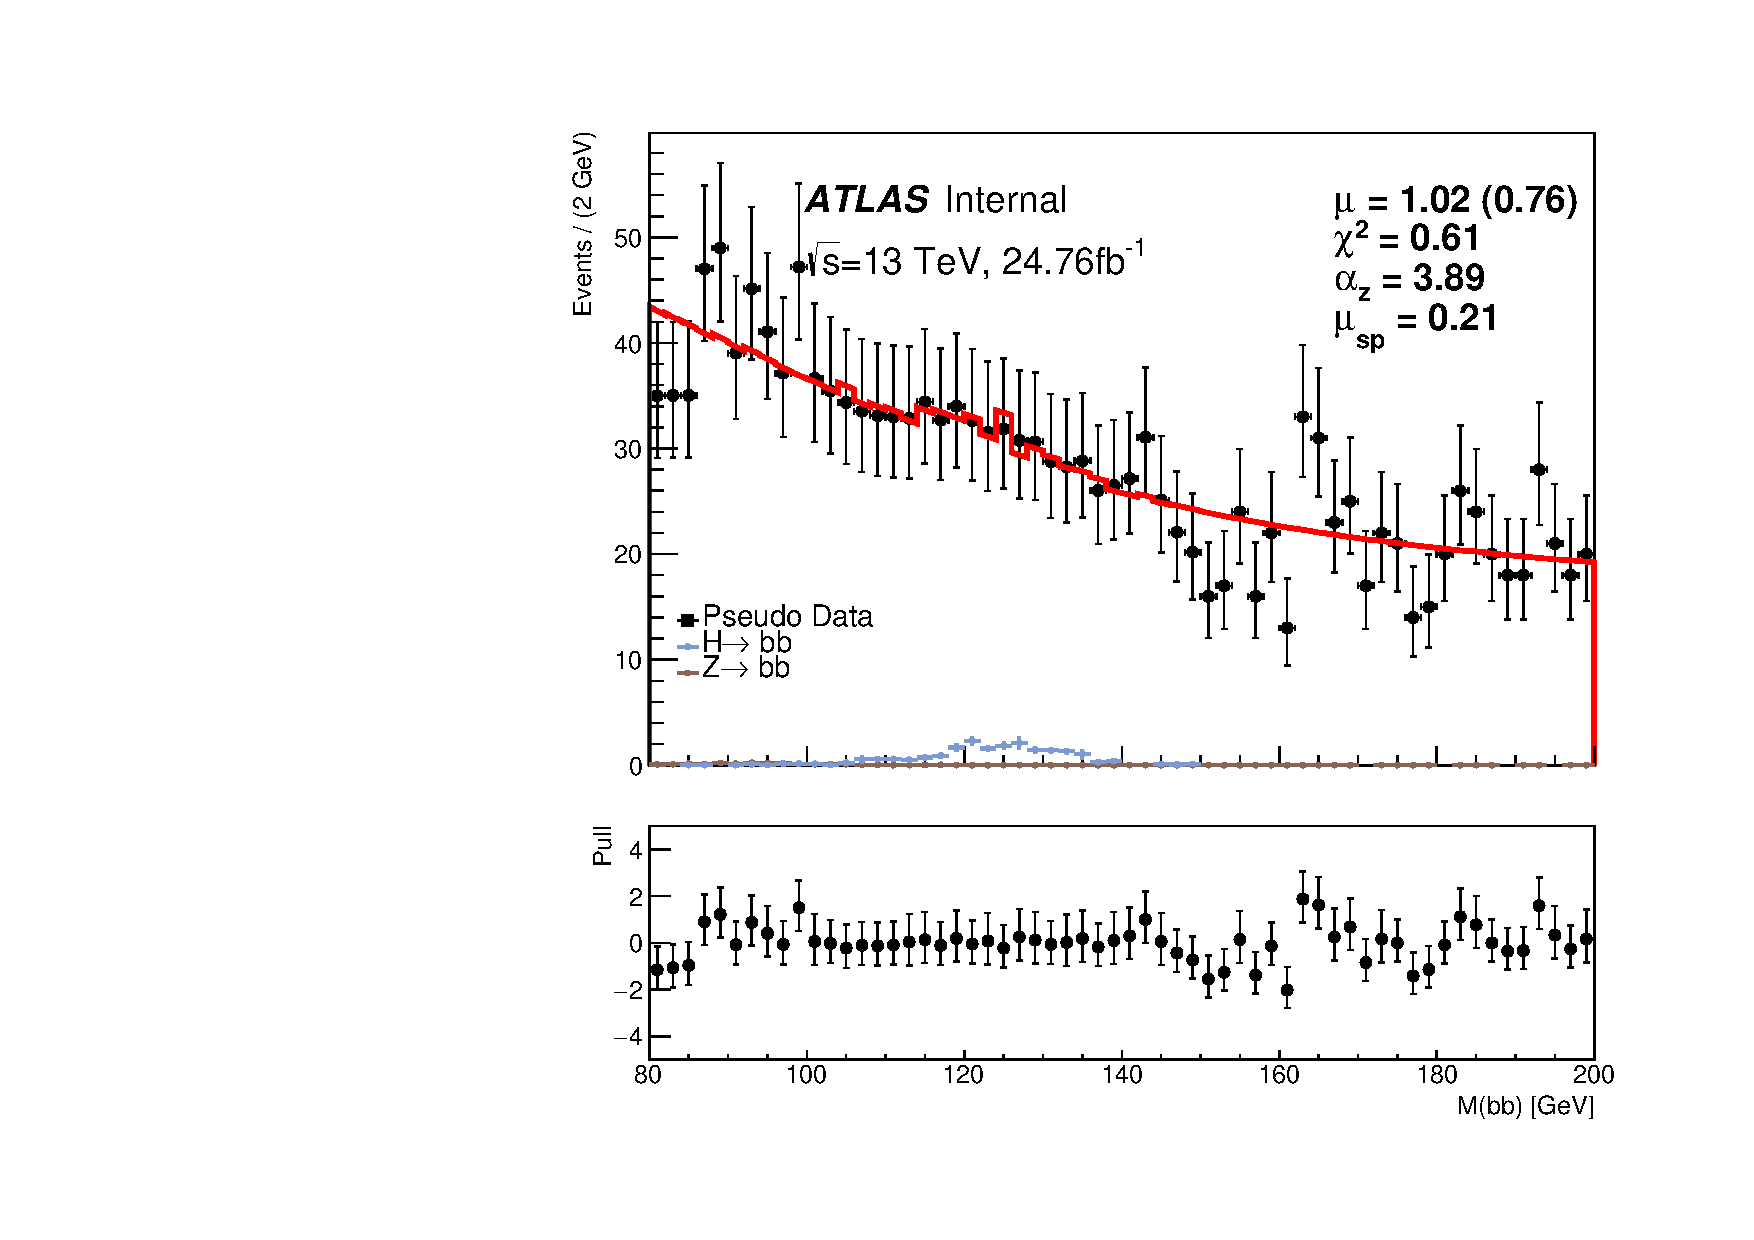
\includegraphics[width=0.48\textwidth]{figures/FitCombined/zfloat_testVBF_ICHEP_2cen_SRI.pdf}
% 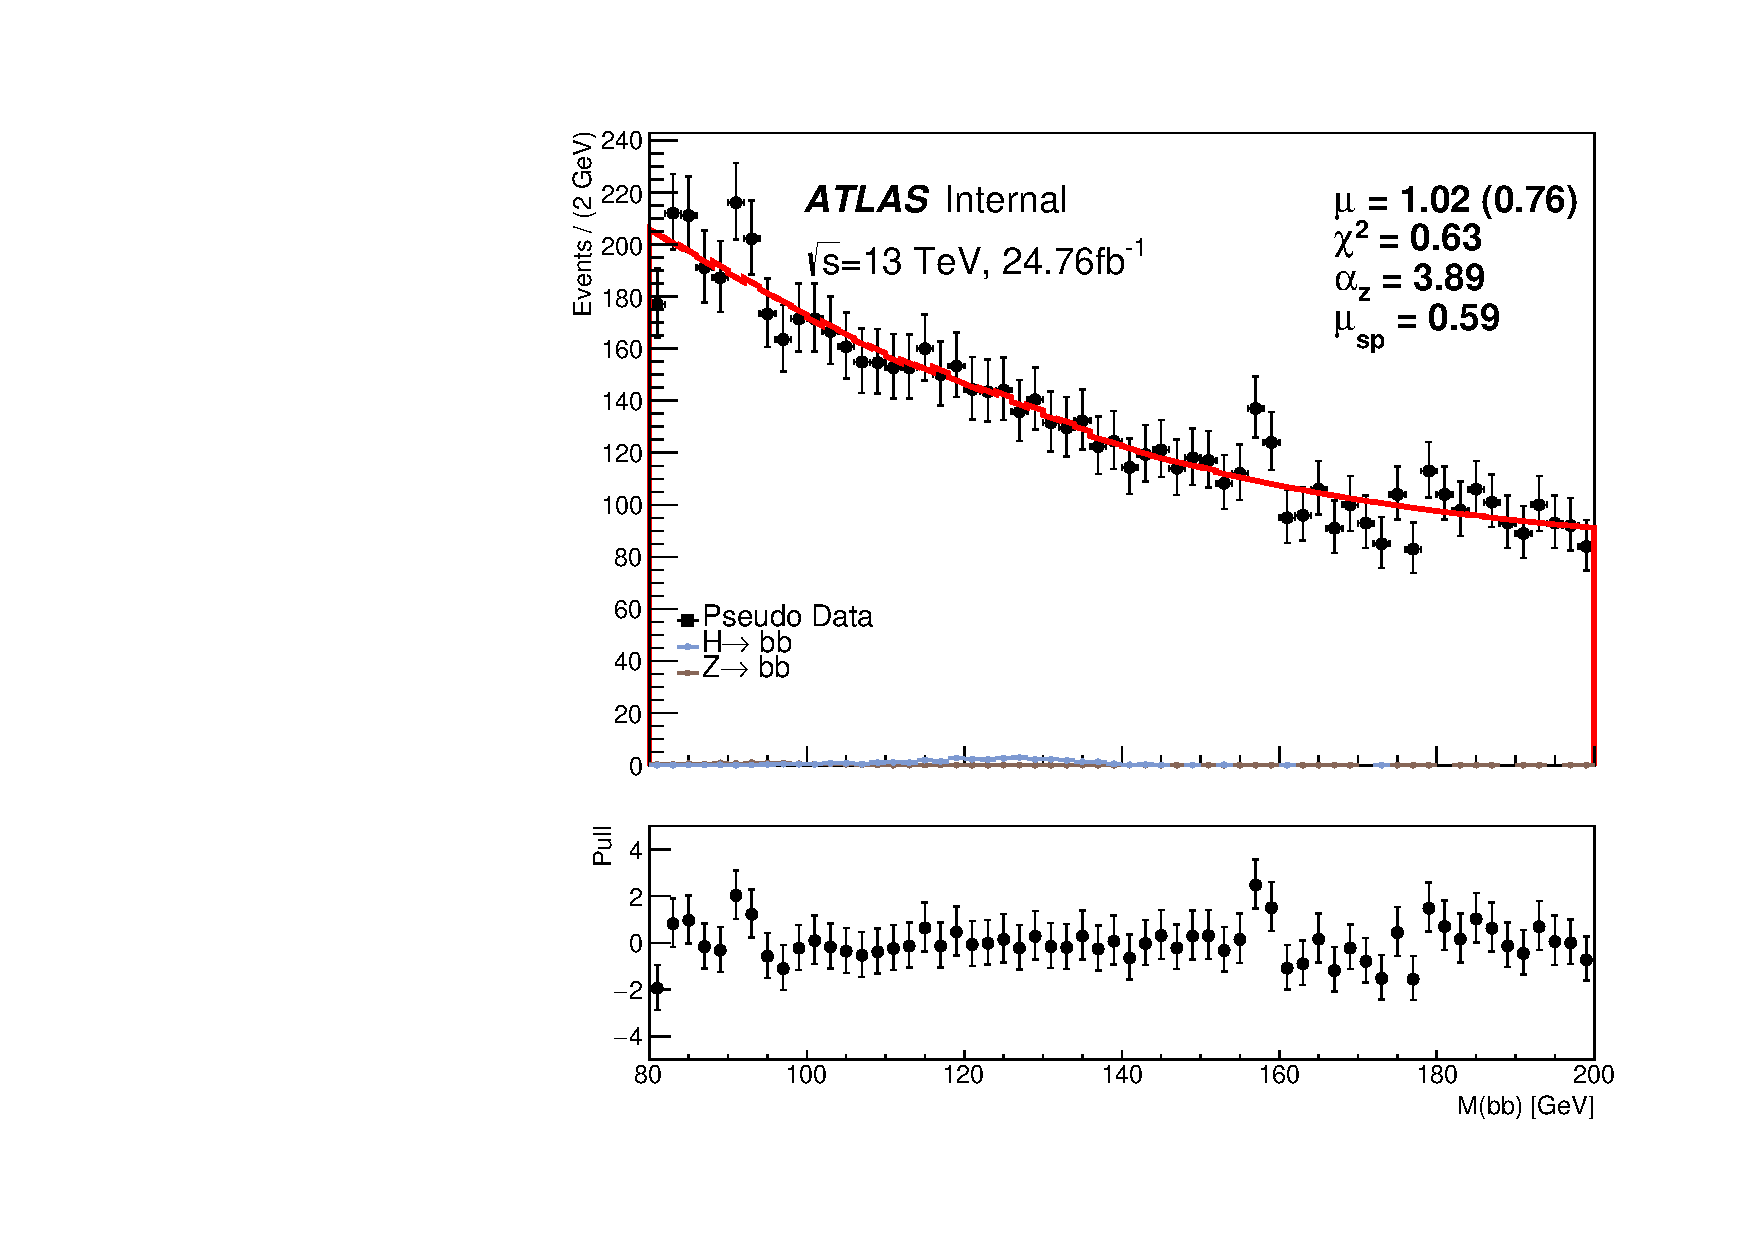
\includegraphics[width=0.48\textwidth]{figures/FitCombined/zfloat_testVBF_ICHEP_2cen_SRII.pdf}\\
% 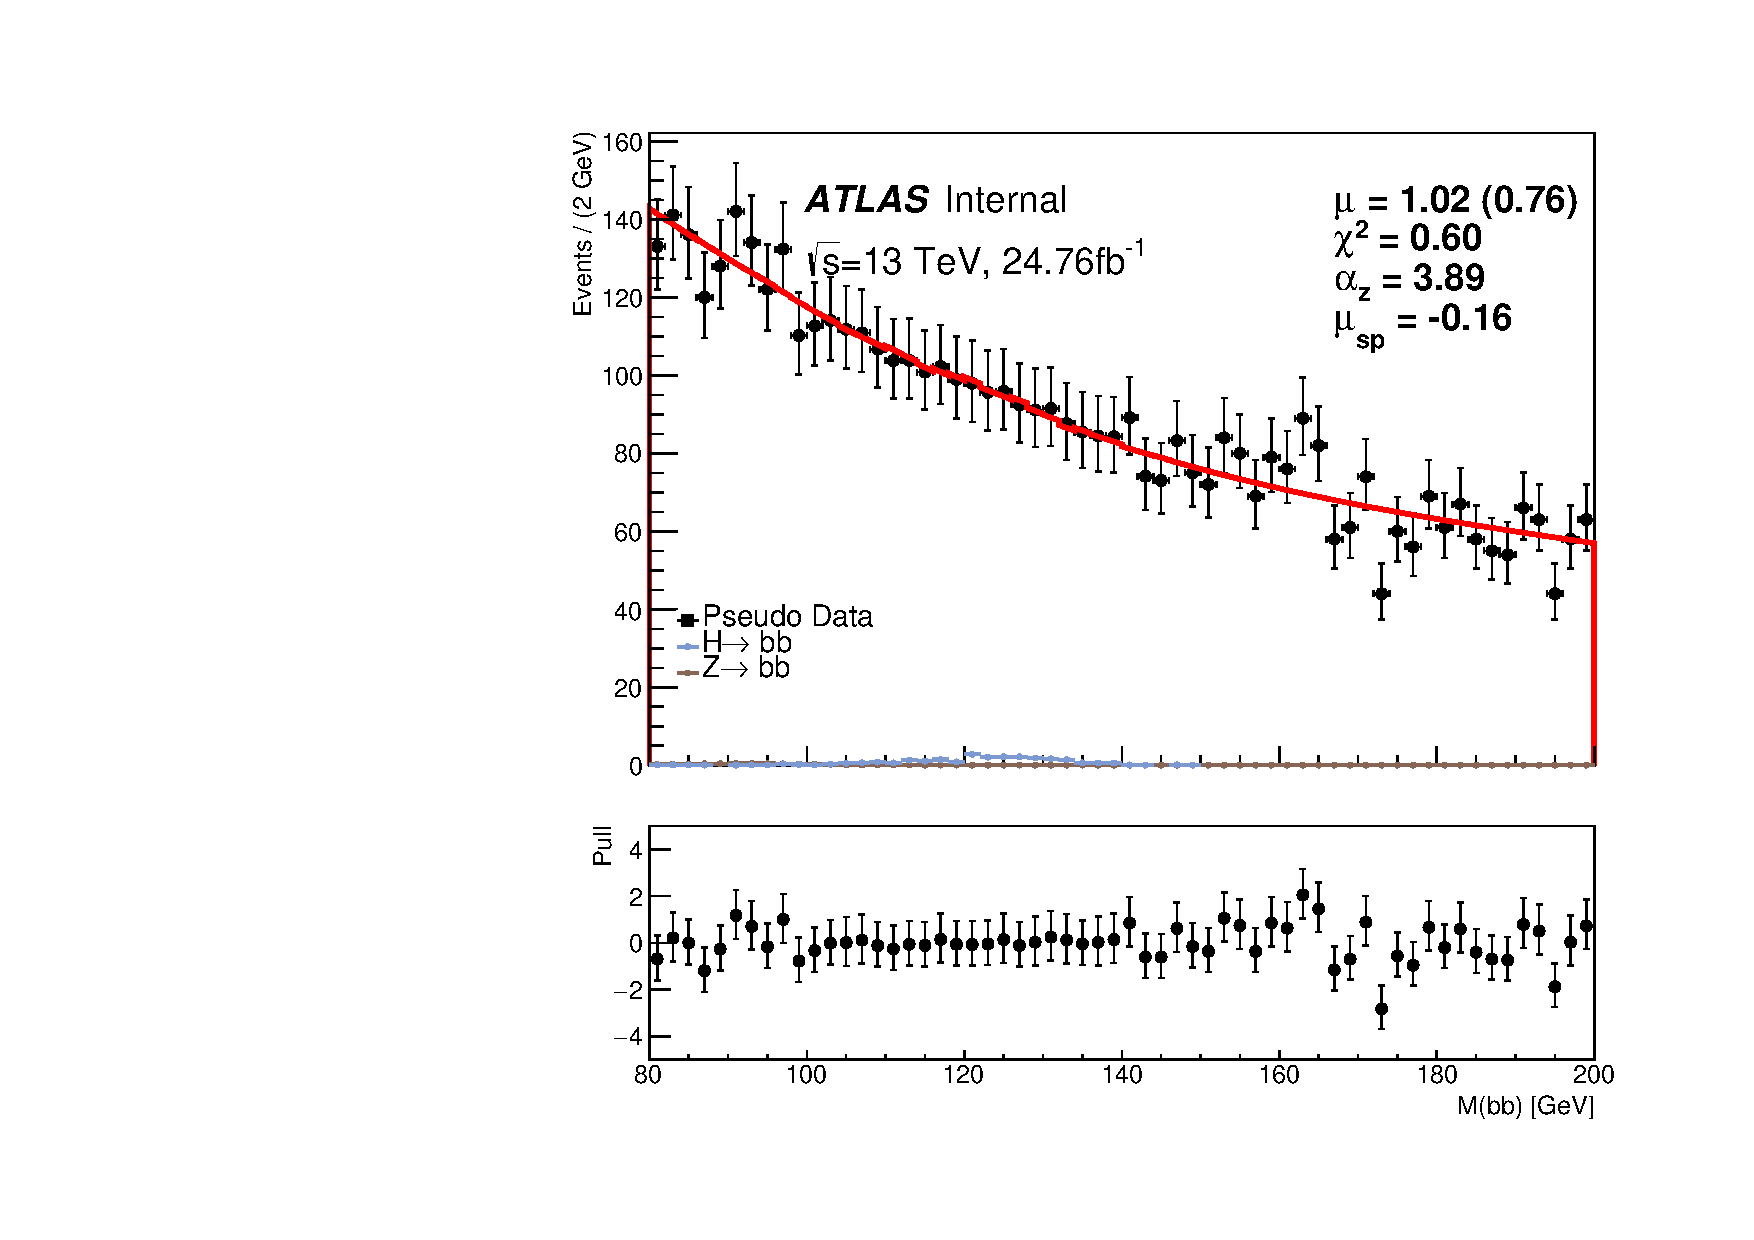
\includegraphics[width=0.48\textwidth]{figures/FitCombined/zfloat_testVBF_ICHEP_4cen_SRI.pdf}
% 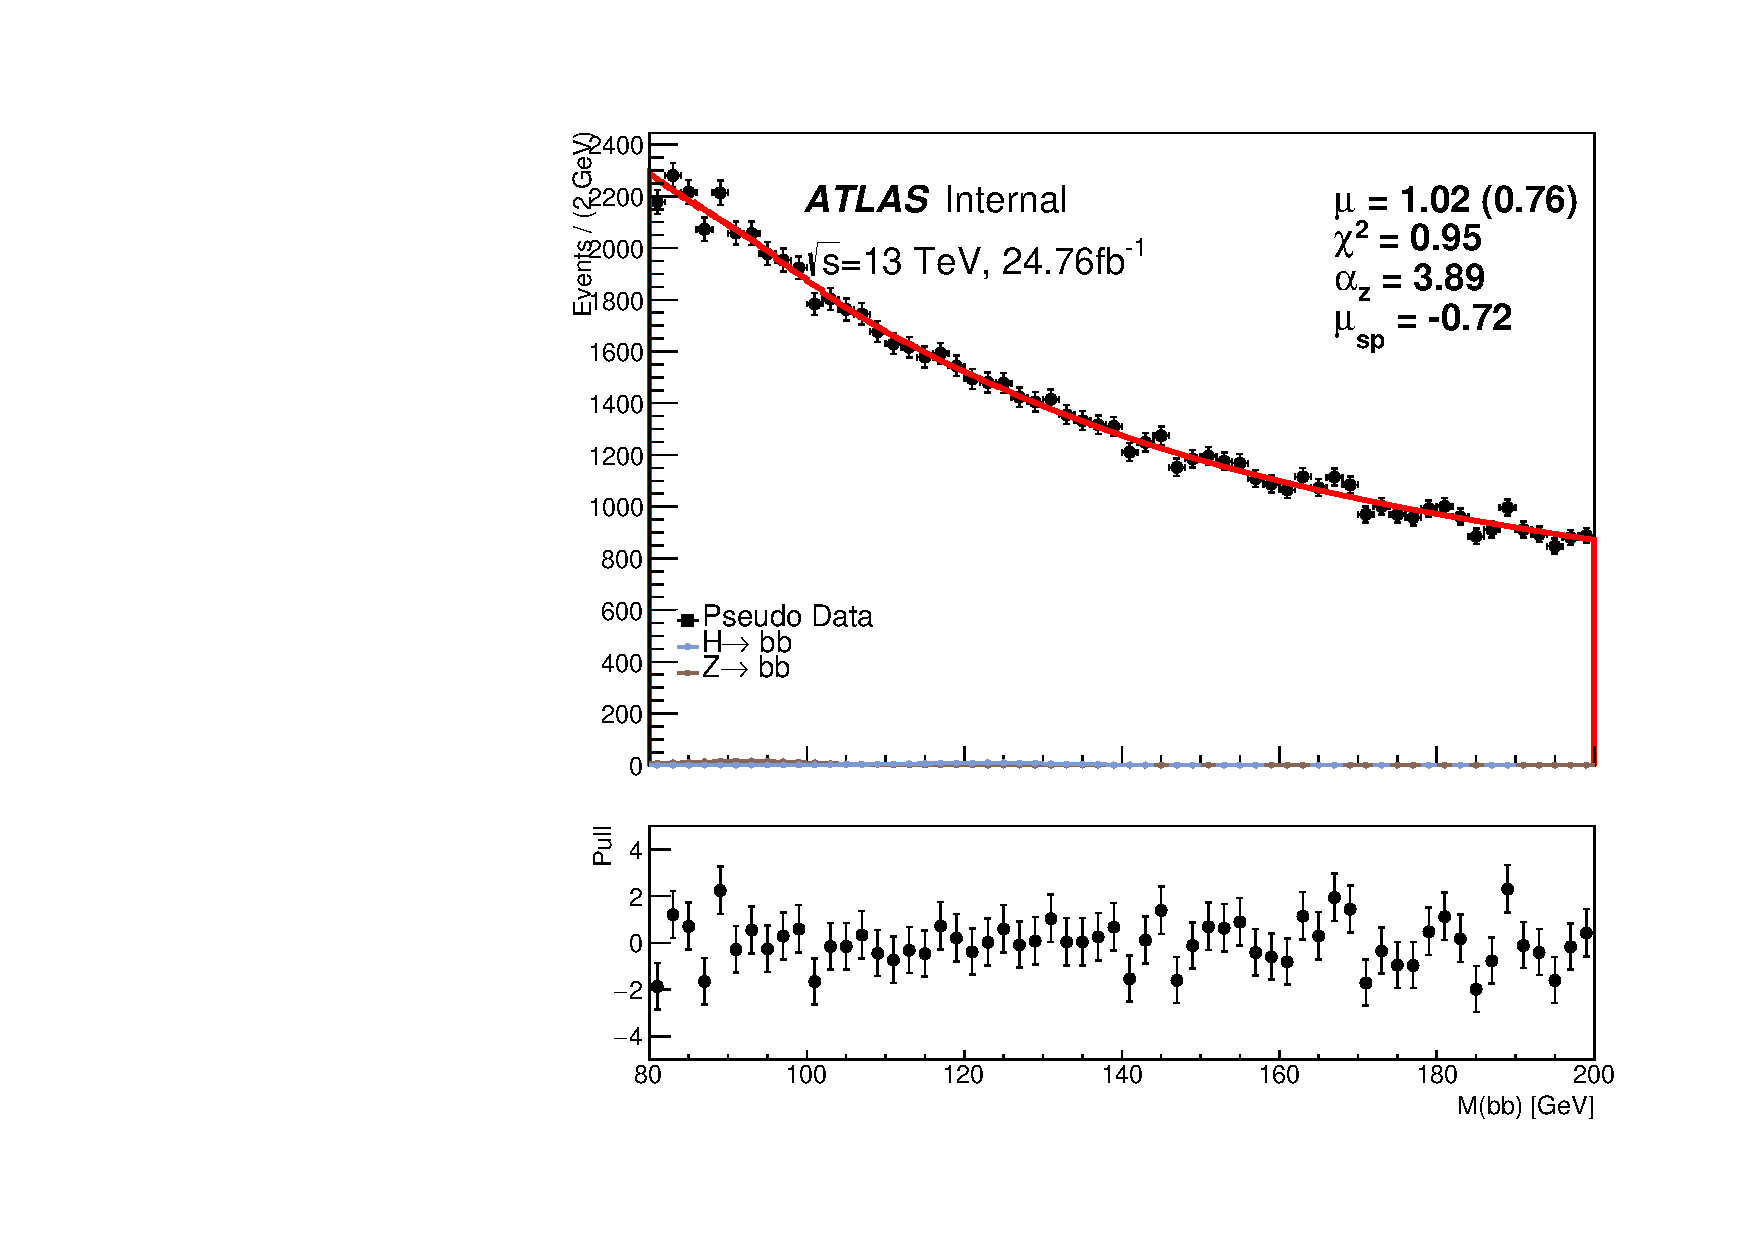
\includegraphics[width=0.48\textwidth]{figures/FitCombined/zfloat_testVBF_ICHEP_4cen_SRII.pdf}\\
%
%\caption{Pseudo data fit for both channels while the $Z\rightarrow b \bar b$ normalization is left to float. Fits of SR I (left) and SR II (right) for 2 central (top) and 4 central (bottom) are shown.}
%  \label{fig:Fit_combined_znorm}
%\end{figure}
%
%
%\begin{table}[]
%\centering
%  \caption{Z normalization nuisance parameters.  $2cen$ refers to the \twocentral regions, $4cen$ refers to the \fourcentral regions.}
%\label{tab:z_float_all}
%\begin{tabular}{|l|l|}
%\hline
%
%$\alpha_{2cen}(CR)$         & $3.76\pm 4.89$   \\ \hline
%$\alpha_{2cen}(SRI)$        & $52.47\pm 36.78$   \\ \hline
%$\alpha_{2cen}(SRII)$       & $14.63\pm 12.47$   \\ \hline
%$\alpha_{4cen}(CR)$         & $3.63\pm 1.46$   \\ \hline
%$\alpha_{4cen}(SRI)$        & $16.69\pm 50.76$   \\ \hline
%$\alpha_{4cen}(SRII)$       & $5.53\pm 2.95$   \\ \hline
%
%
%\end{tabular}
%\end{table}
%
%
%\begin{figure}[htbp]
%  \centering
% 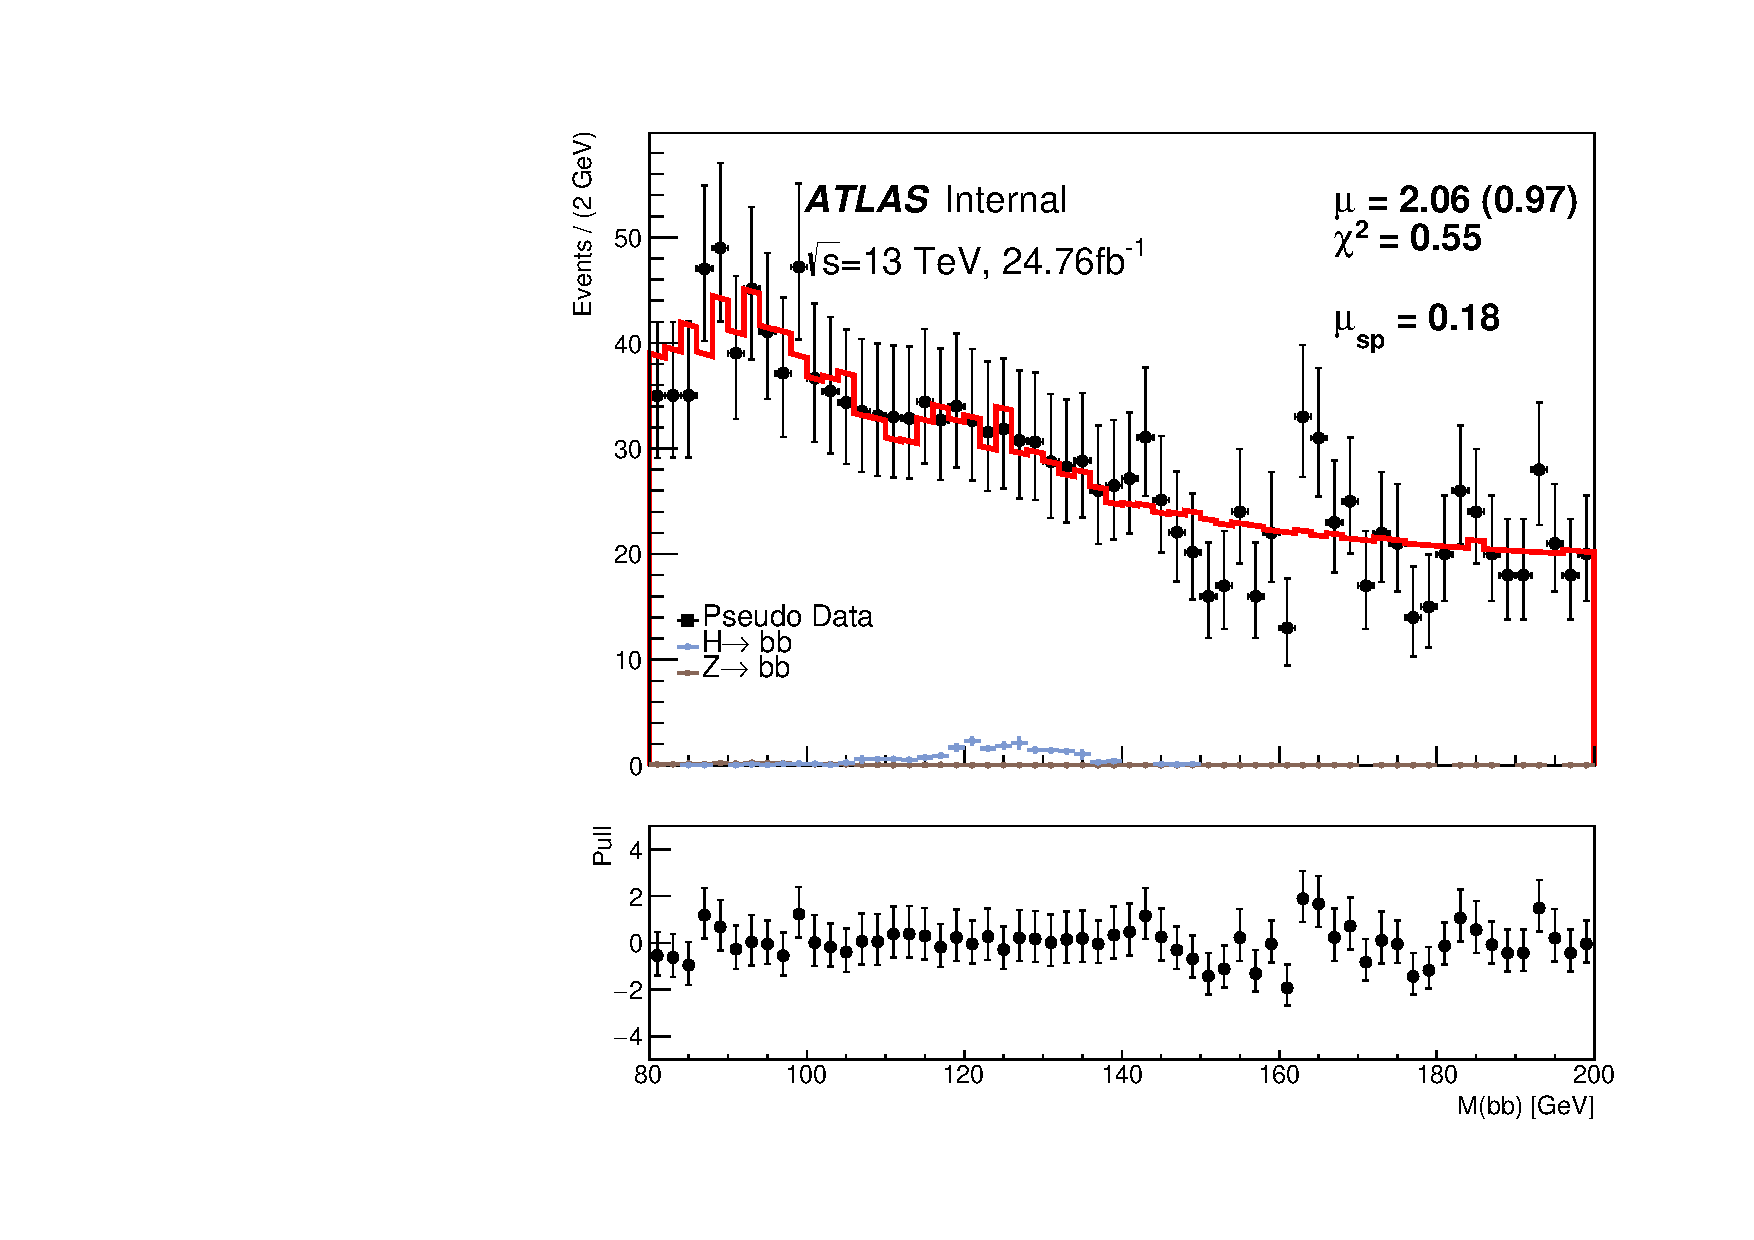
\includegraphics[width=0.48\textwidth]{figures/FitCombined/zfloatall_testVBF_ICHEP_2cen_SRI.pdf}
% 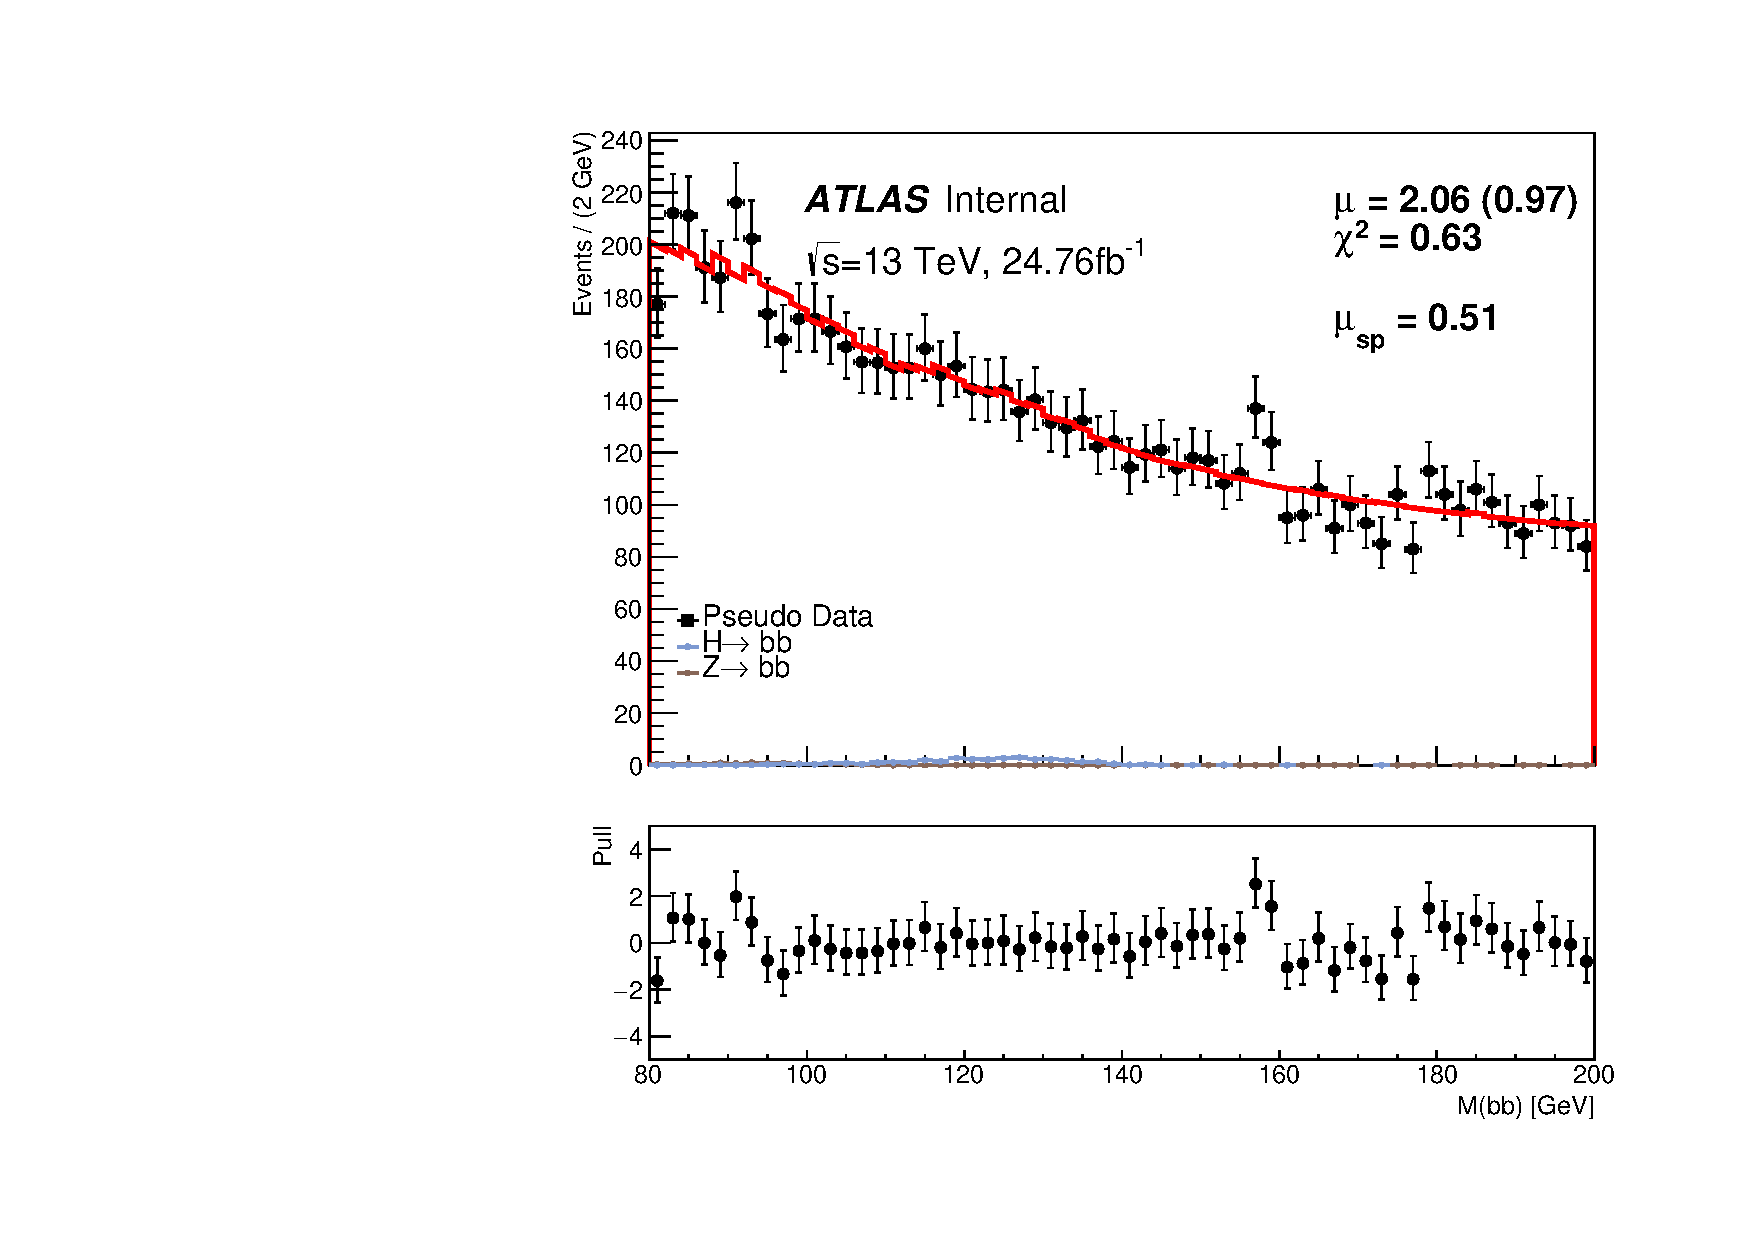
\includegraphics[width=0.48\textwidth]{figures/FitCombined/zfloatall_testVBF_ICHEP_2cen_SRII.pdf}\\
% 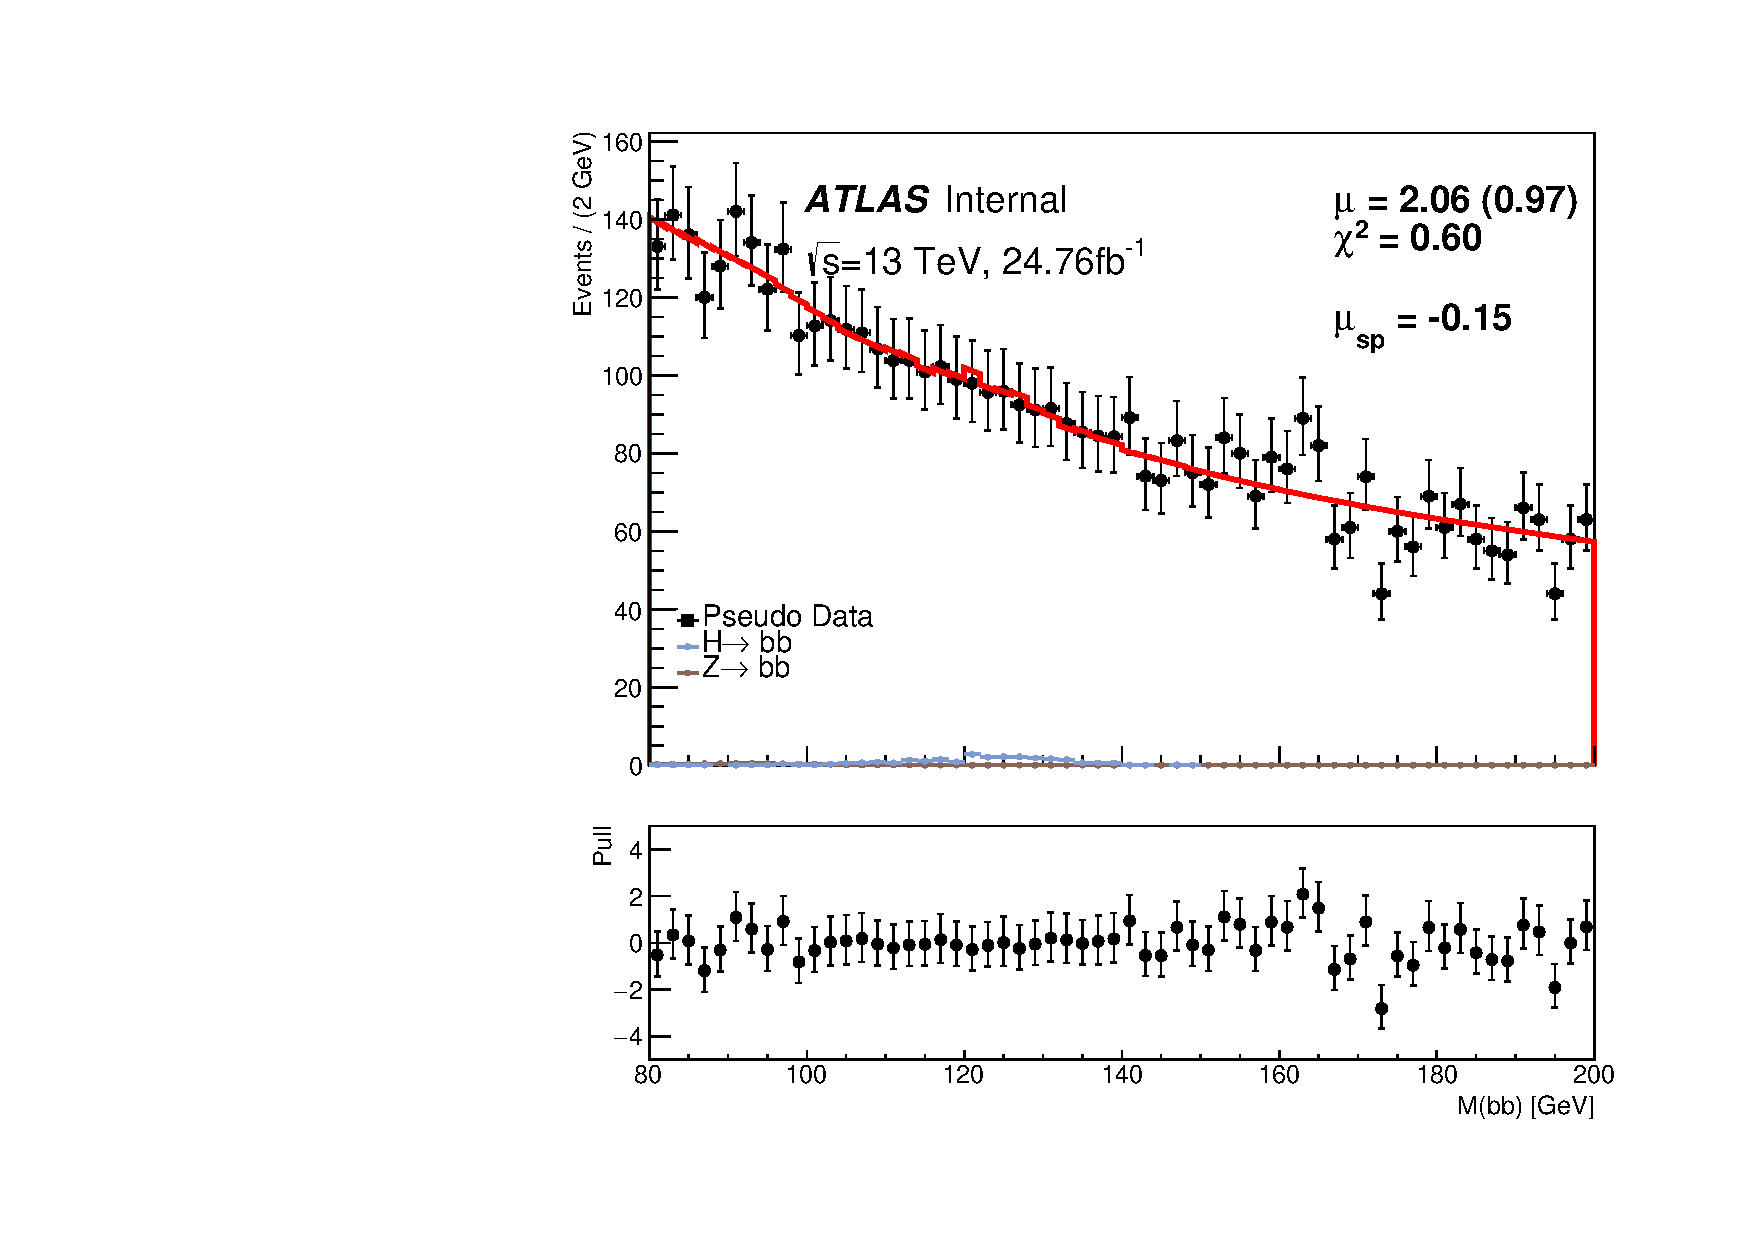
\includegraphics[width=0.48\textwidth]{figures/FitCombined/zfloatall_testVBF_ICHEP_4cen_SRI.pdf}
% 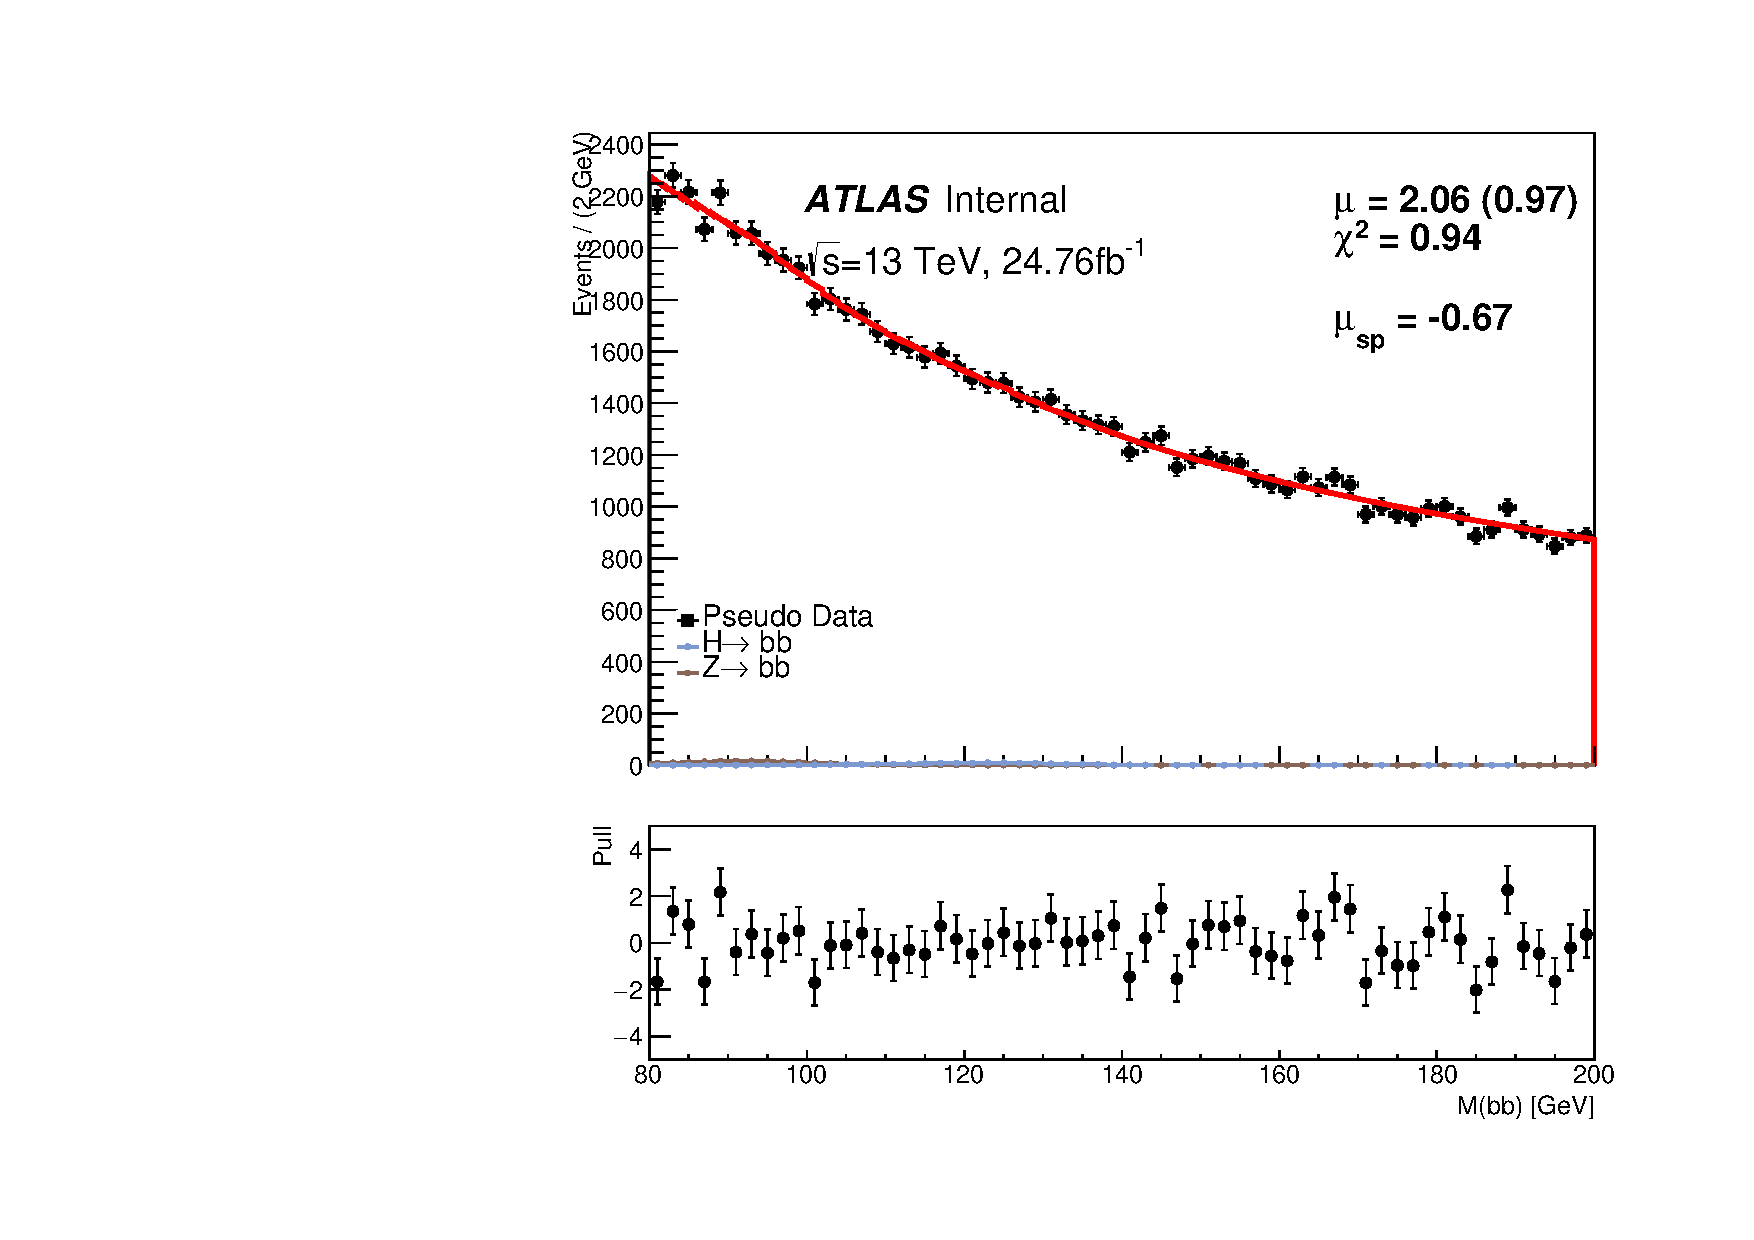
\includegraphics[width=0.48\textwidth]{figures/FitCombined/zfloatall_testVBF_ICHEP_4cen_SRII.pdf}\\
%
%\caption{Pseudo data fit for both channels while the $Z\rightarrow b \bar b$ normalizations in each BDT region are left to float. Fits of SR I (left) and SR II (right) for 2 central (top) and 4 central (bottom) are shown.}
%  \label{fig:Fit_combined_znorm_floatall}
%\end{figure}


\begin{figure}[htbp]
  \centering
 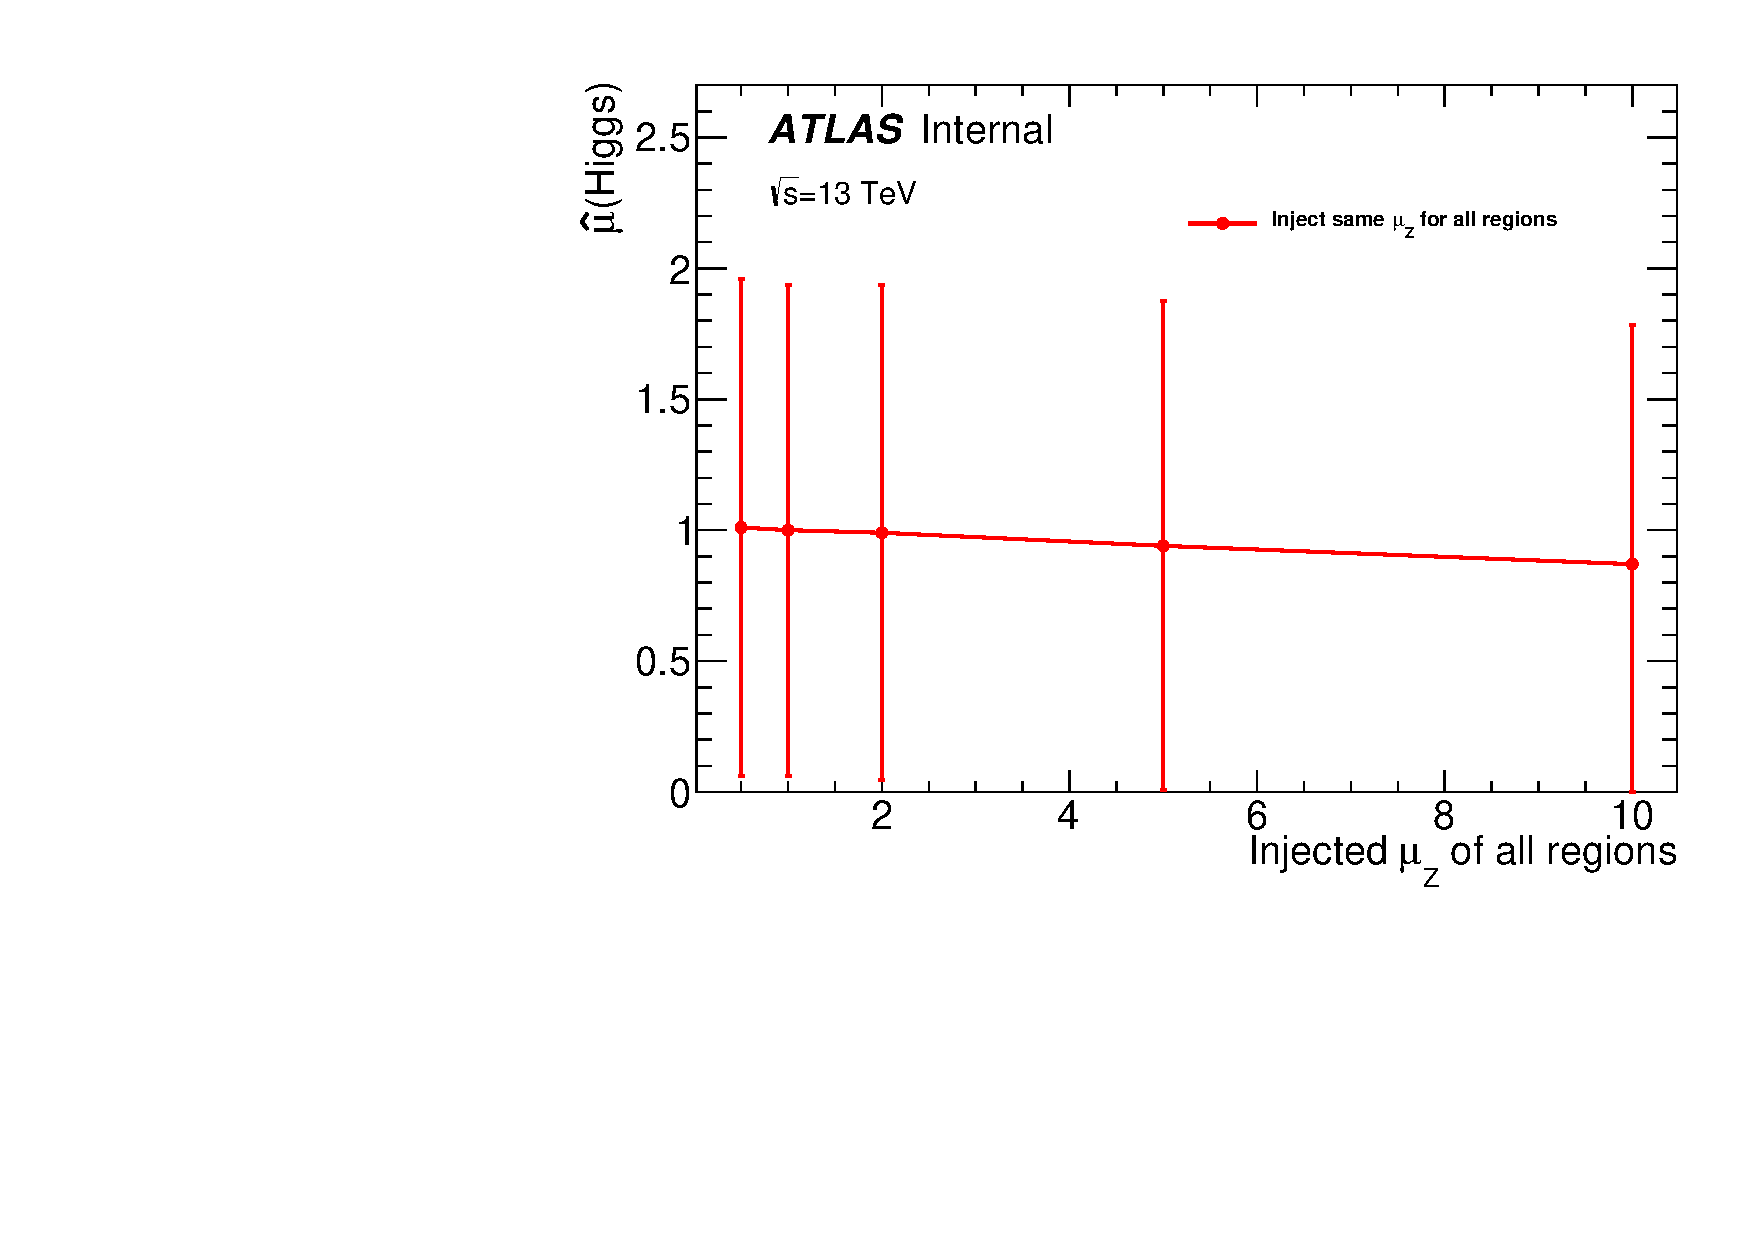
\includegraphics[width=0.48\textwidth]{figures/zstudy/zcon_mu_uniform.pdf}
 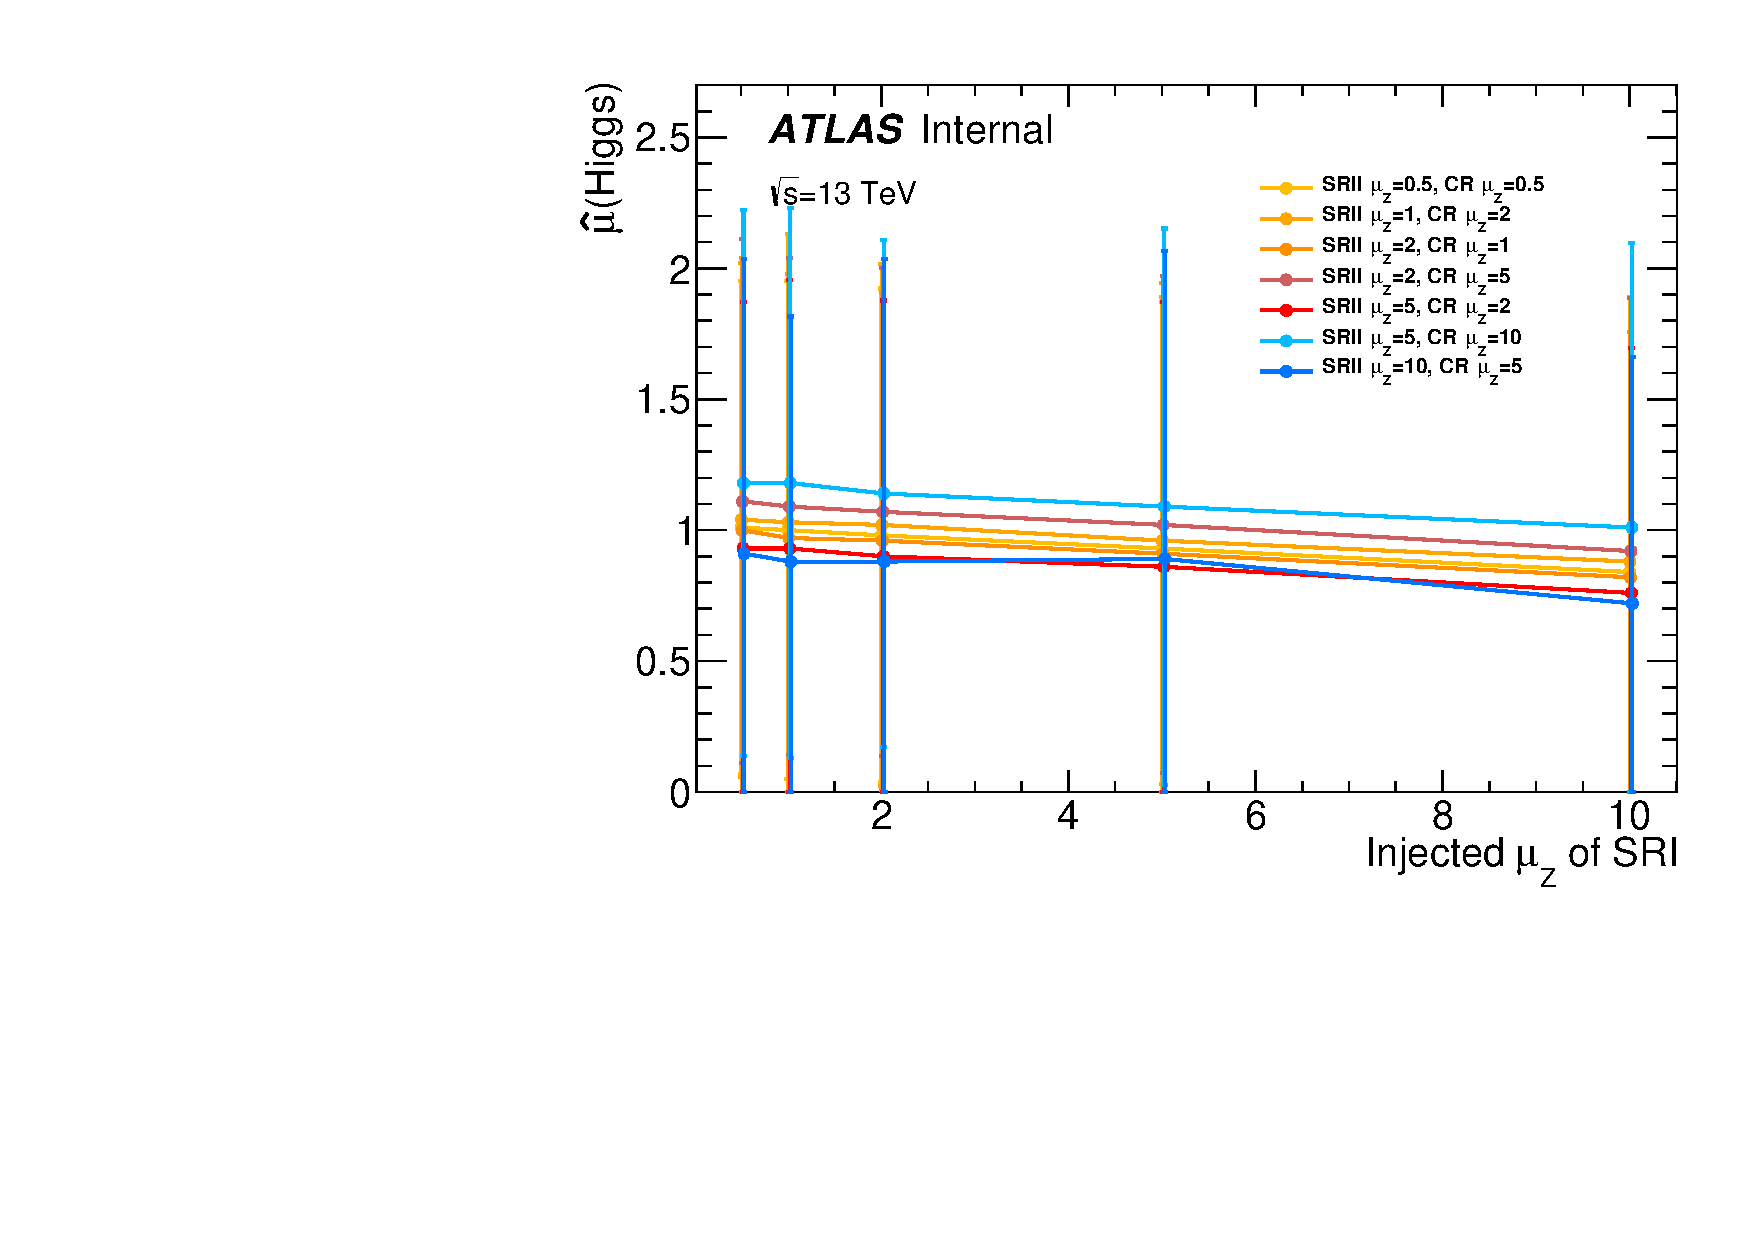
\includegraphics[width=0.48\textwidth]{figures/zstudy/zcon_mu_SRI.pdf}\\
 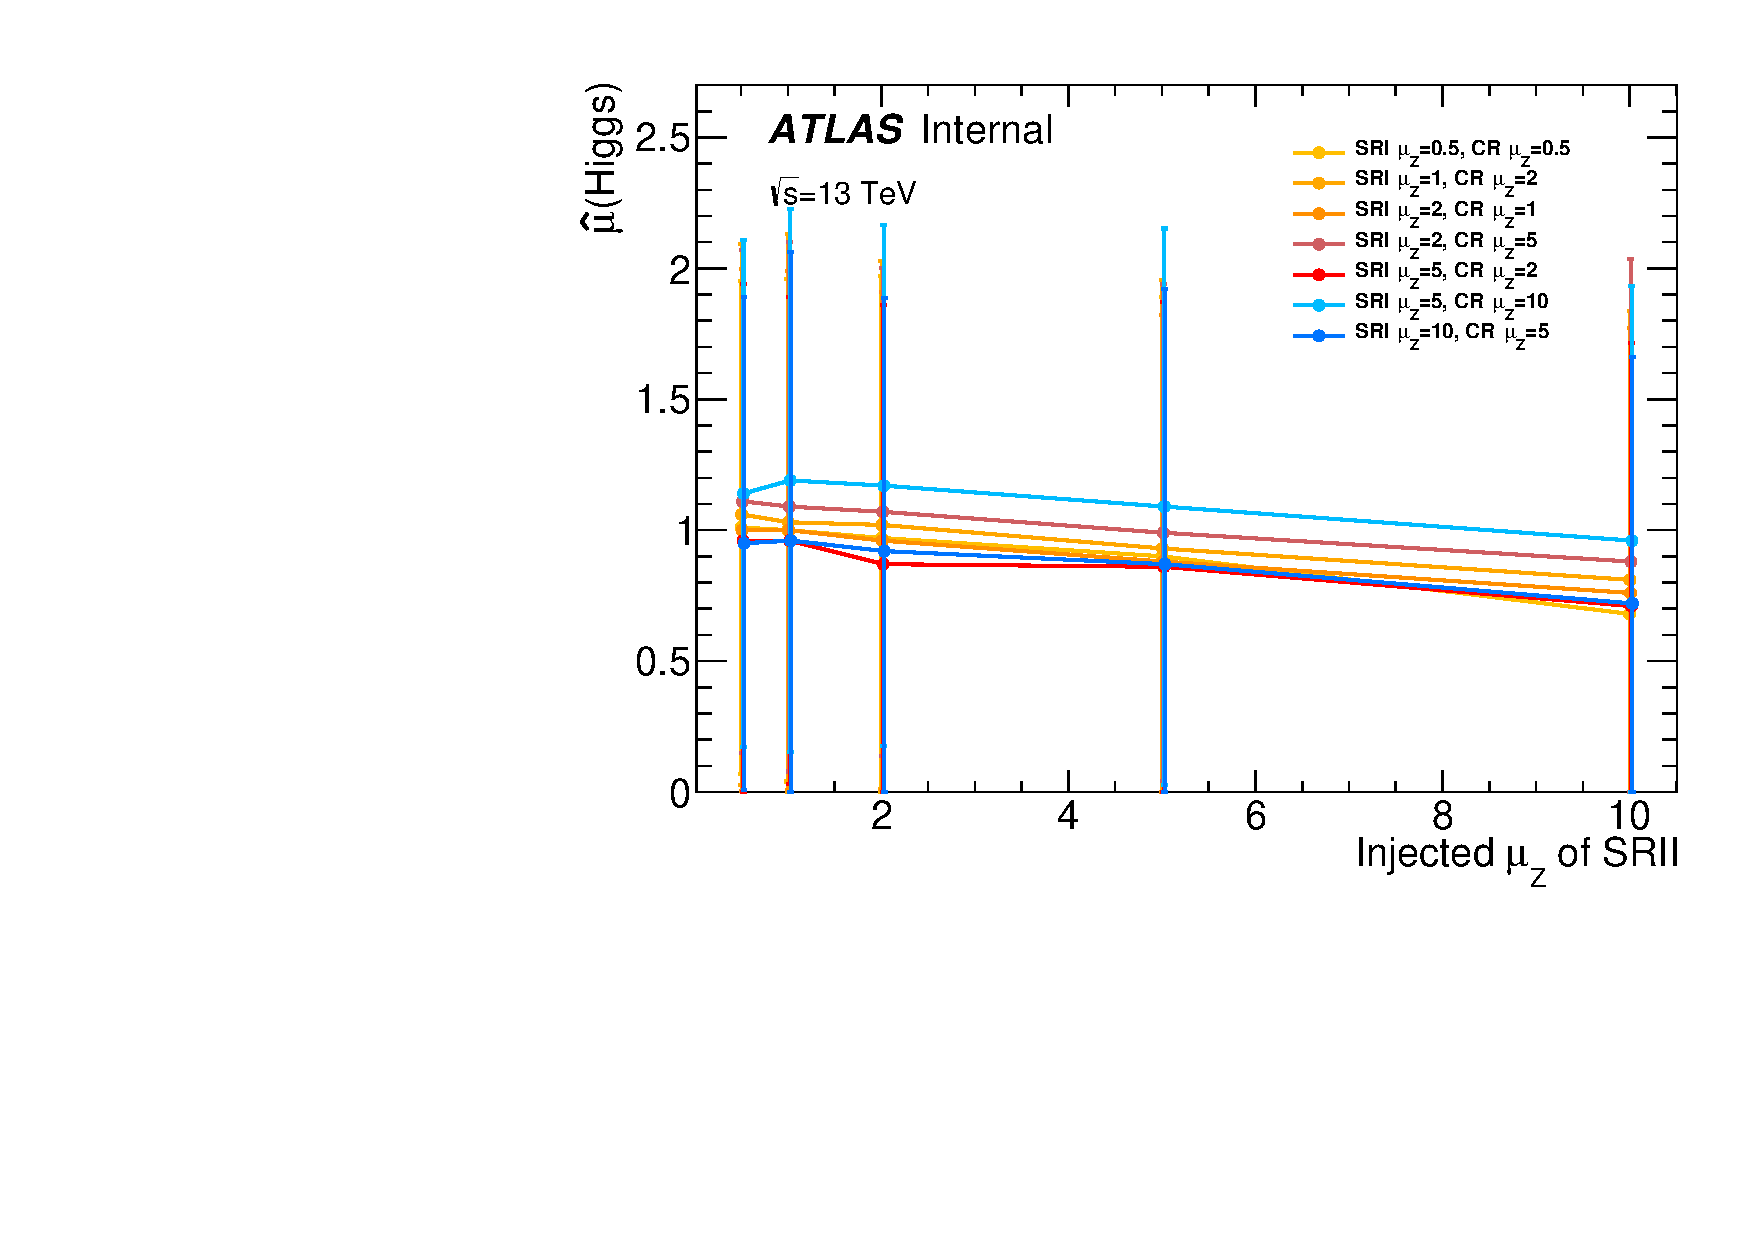
\includegraphics[width=0.48\textwidth]{figures/zstudy/zcon_mu_SRII.pdf}
 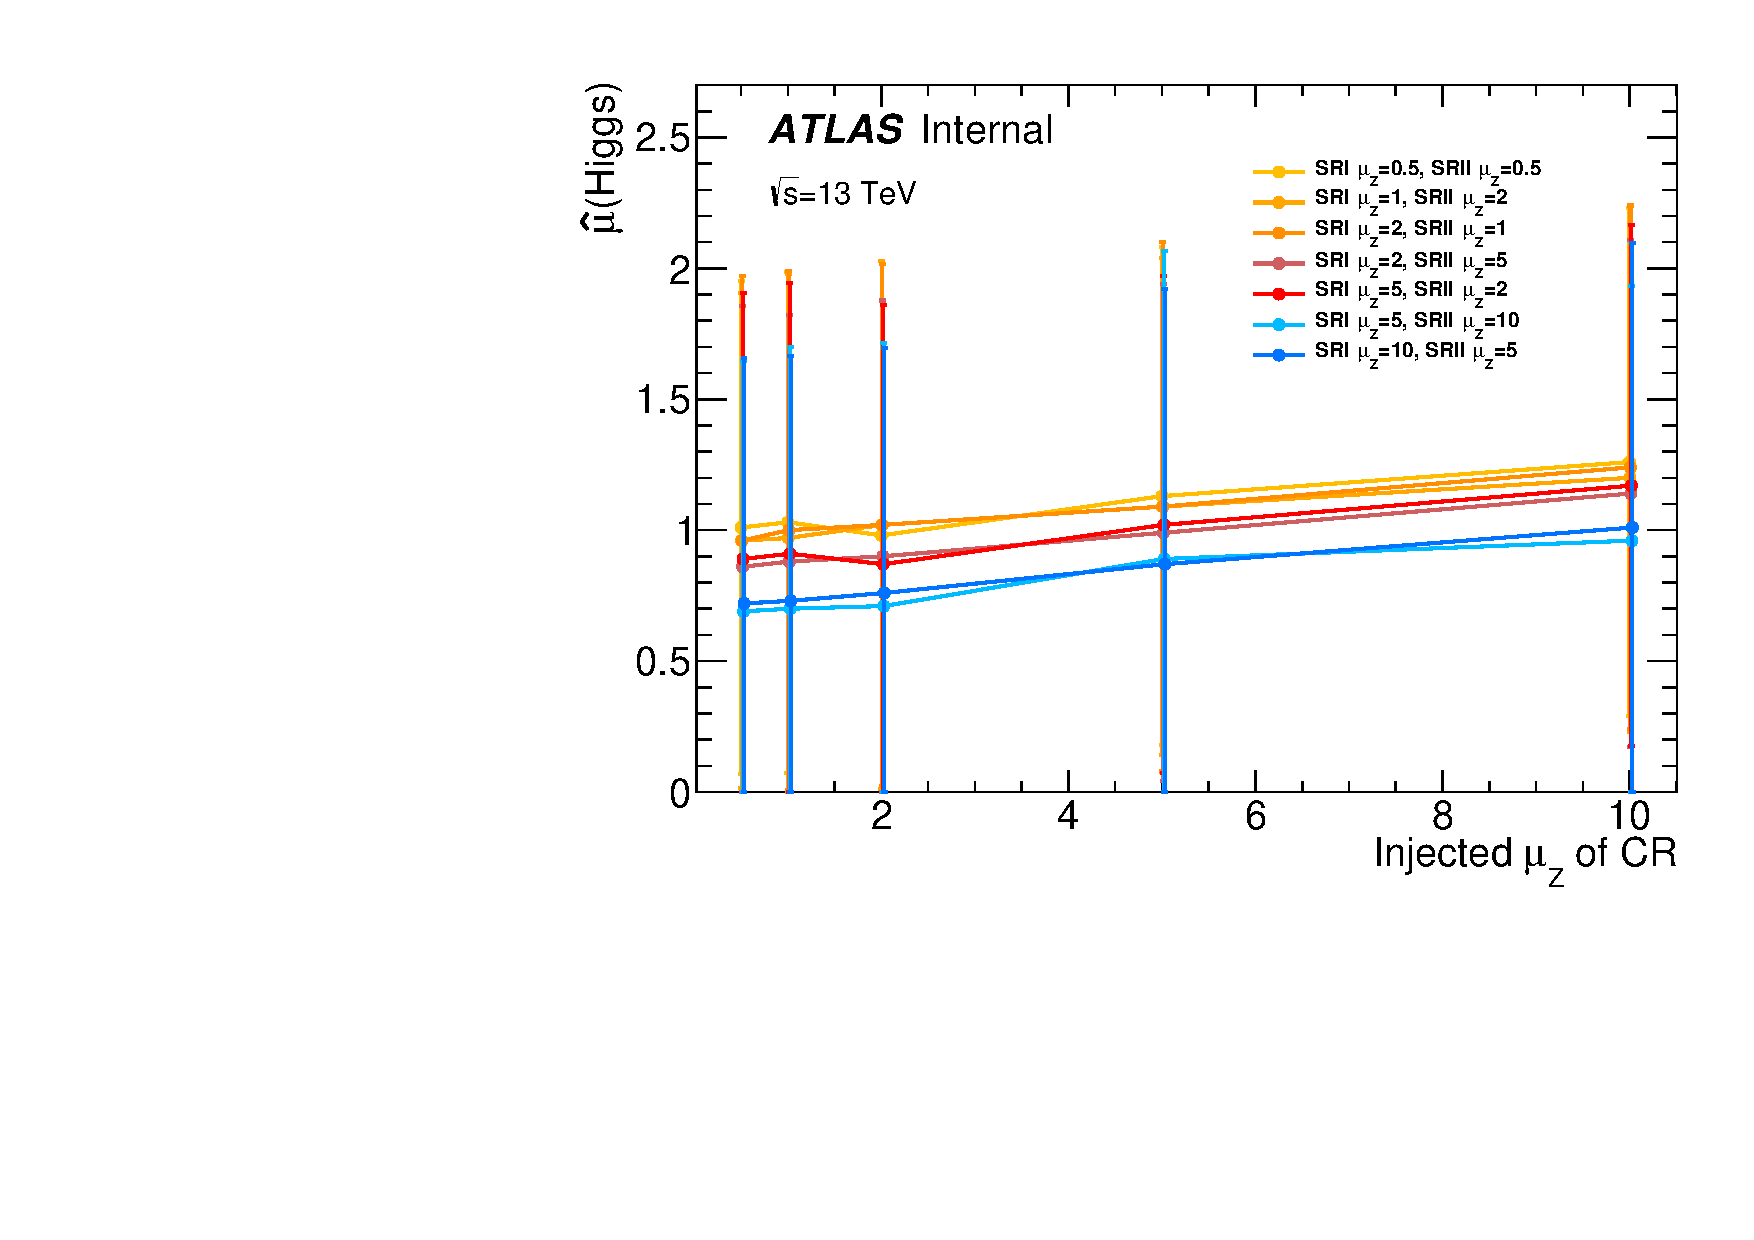
\includegraphics[width=0.48\textwidth]{figures/zstudy/zcon_mu_CR.pdf}\\

\caption{Asimov data fit of Z-injection test applying signle NP with Gaussian prior to the $Z$ normalization in \twocentral channel.}
  \label{fig:zinjection_Con}
\end{figure}


\begin{figure}[htbp]
  \centering
 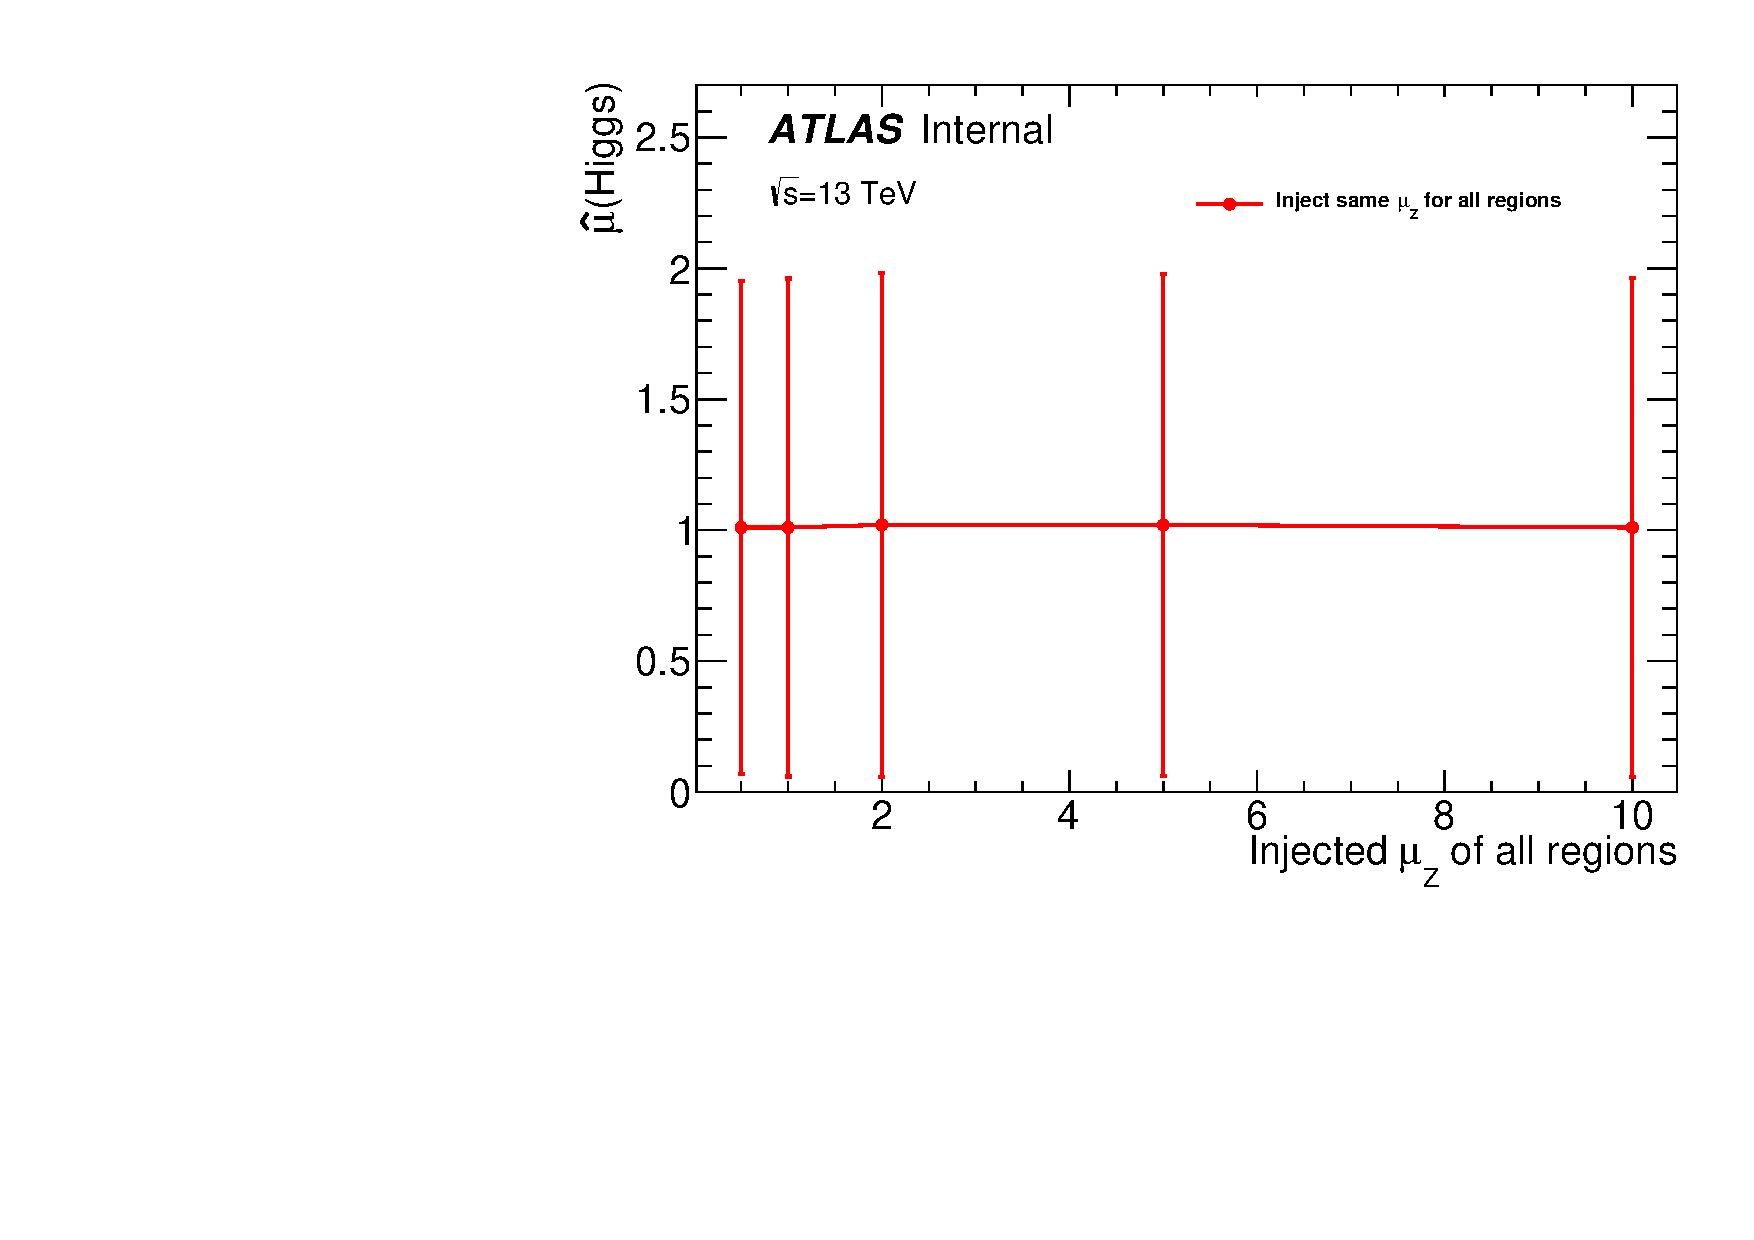
\includegraphics[width=0.48\textwidth]{figures/zstudy/zfloat_mu_uniform.pdf}
 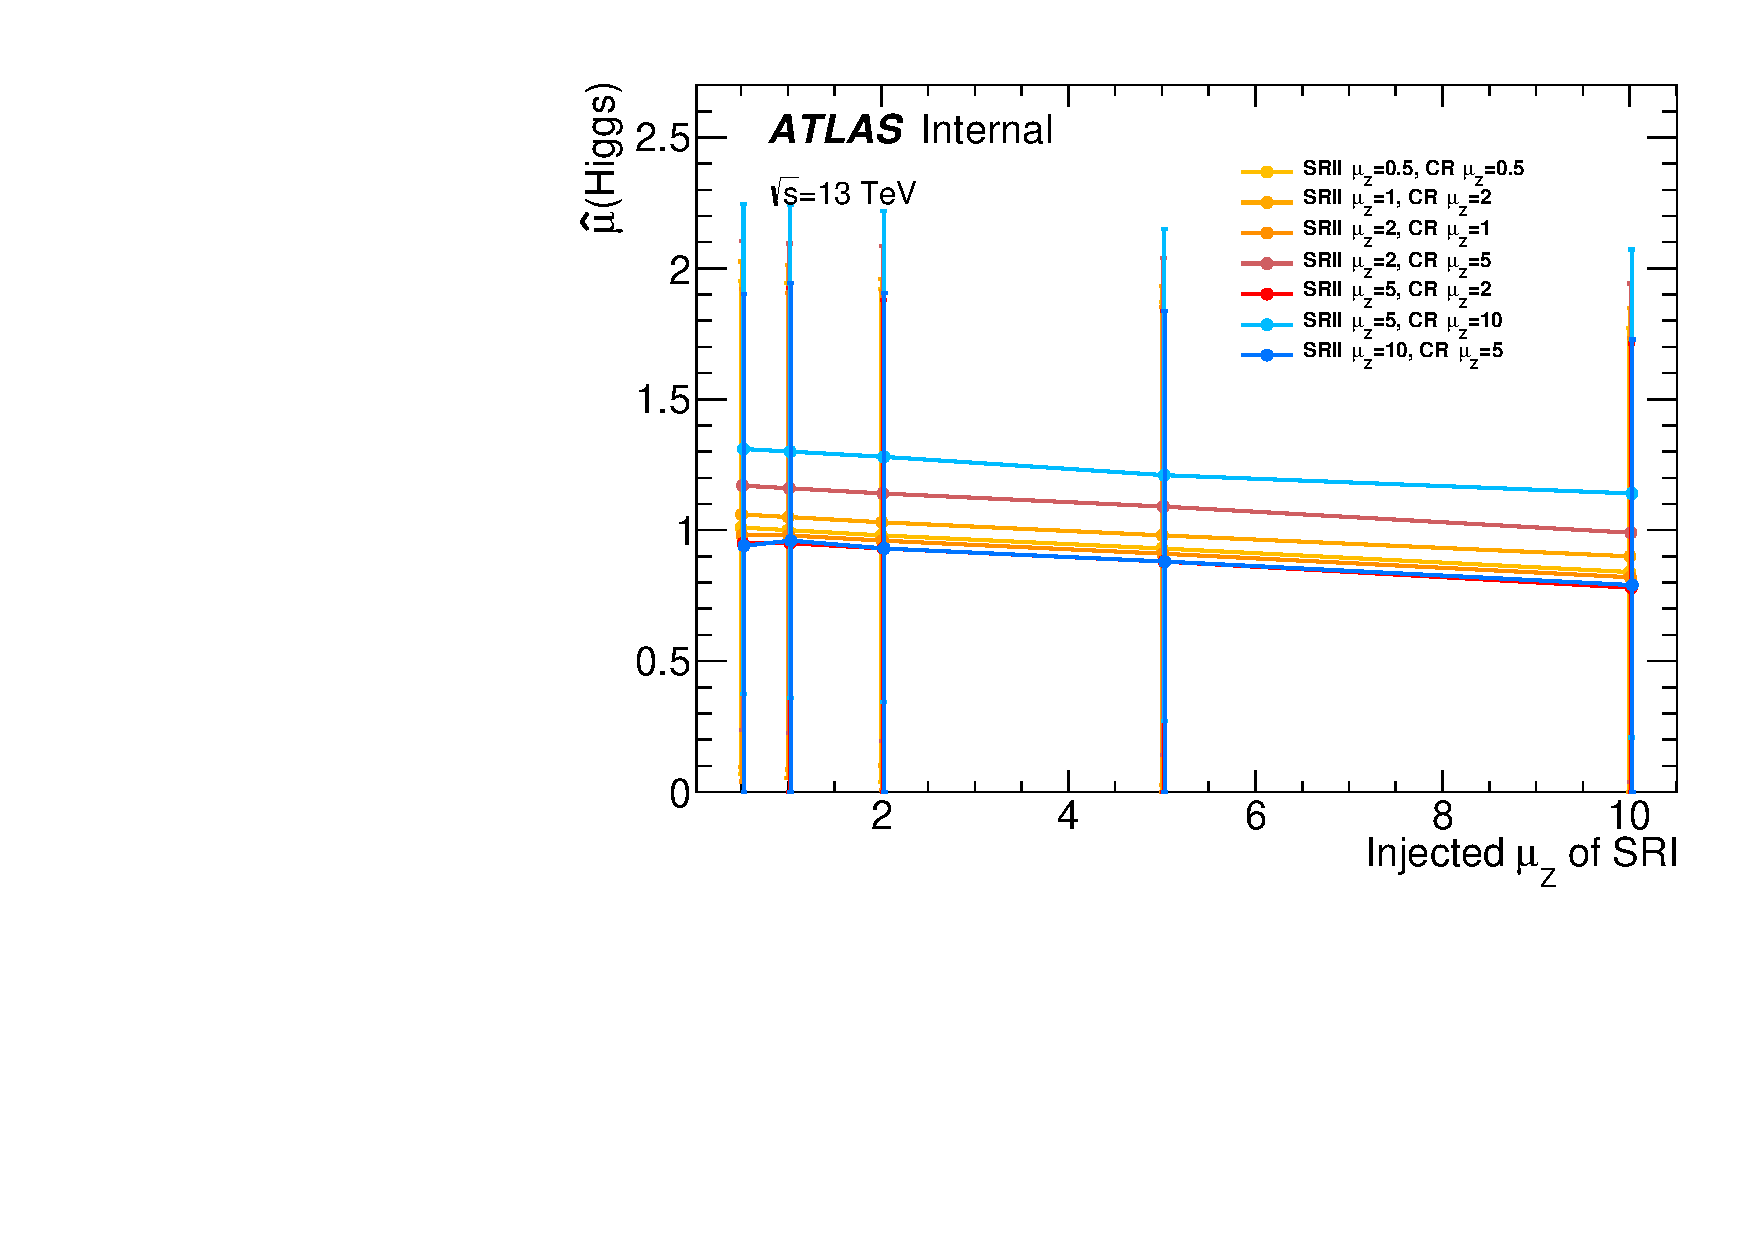
\includegraphics[width=0.48\textwidth]{figures/zstudy/zfloat_mu_SRI.pdf}\\
 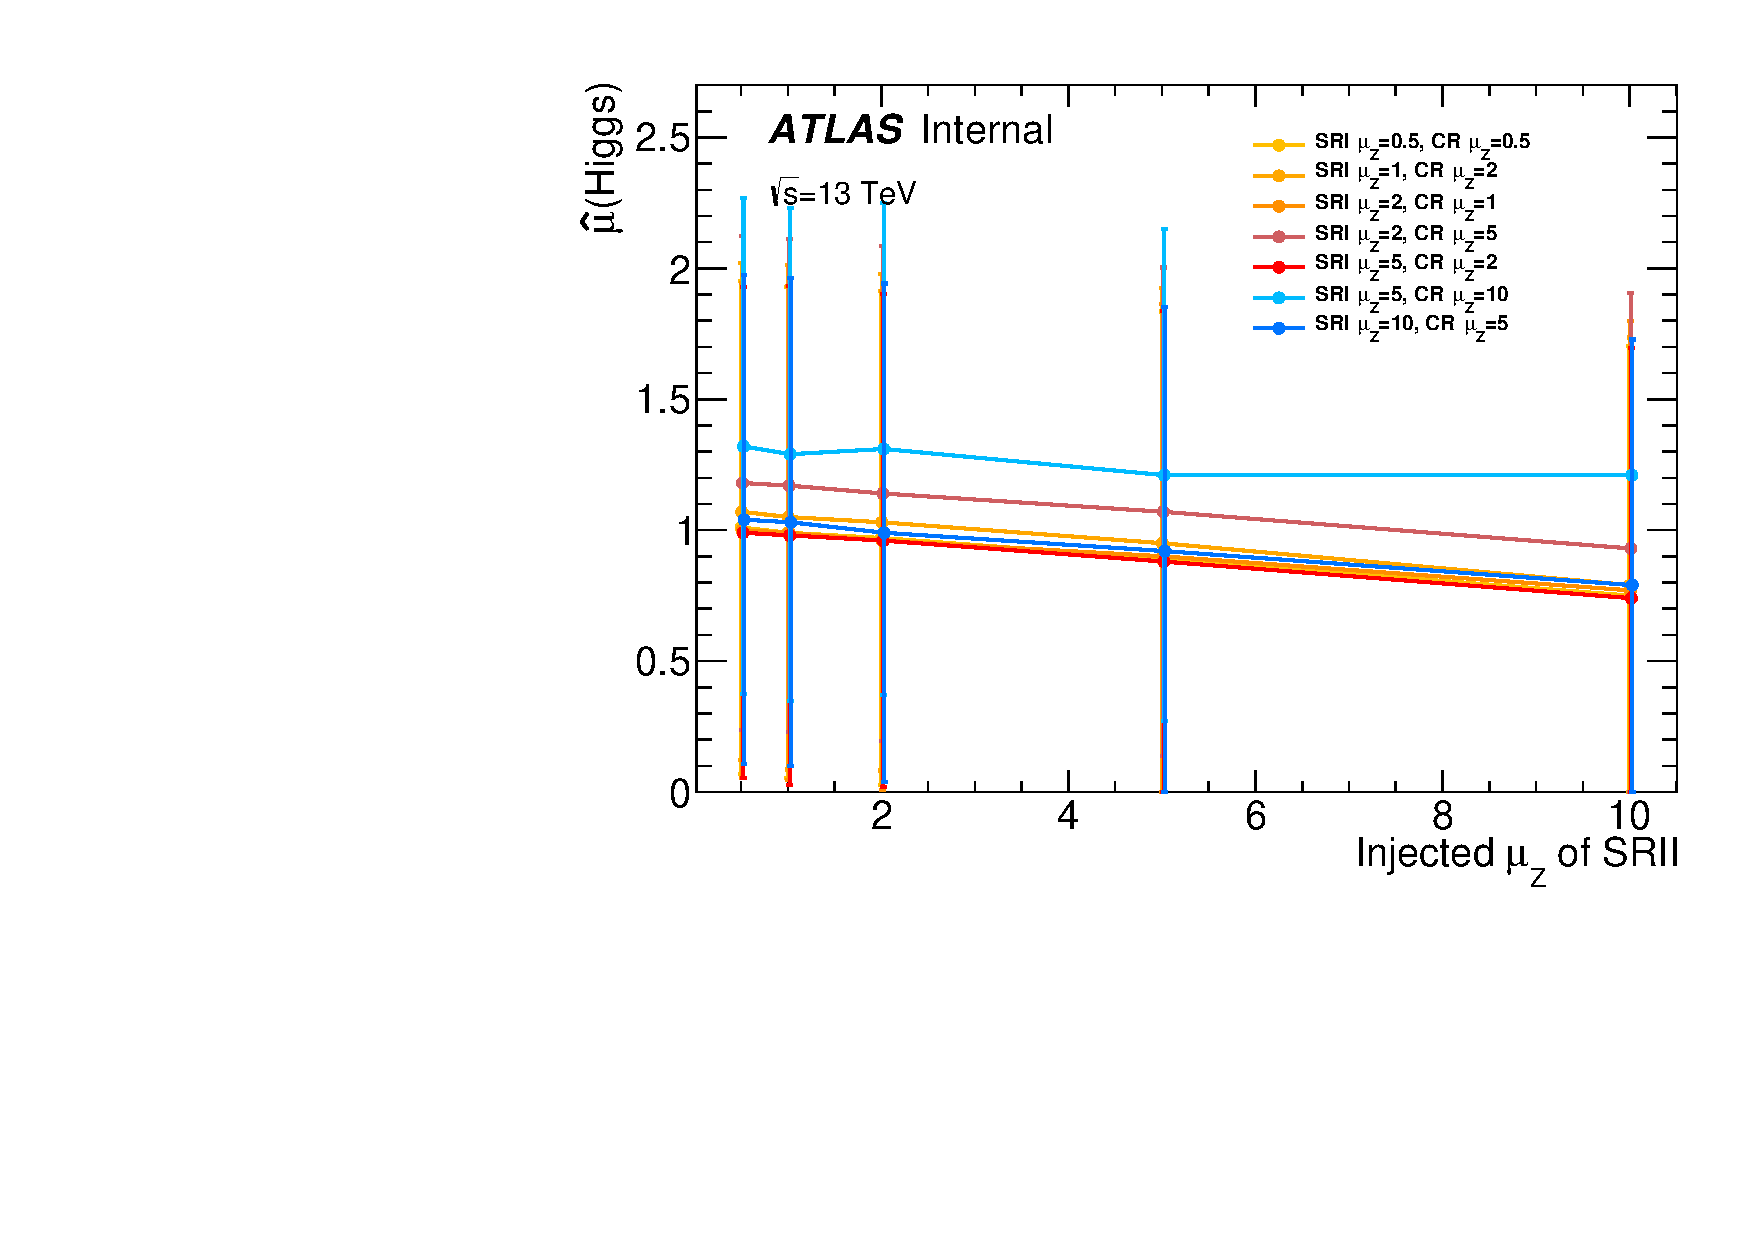
\includegraphics[width=0.48\textwidth]{figures/zstudy/zfloat_mu_SRII.pdf}
 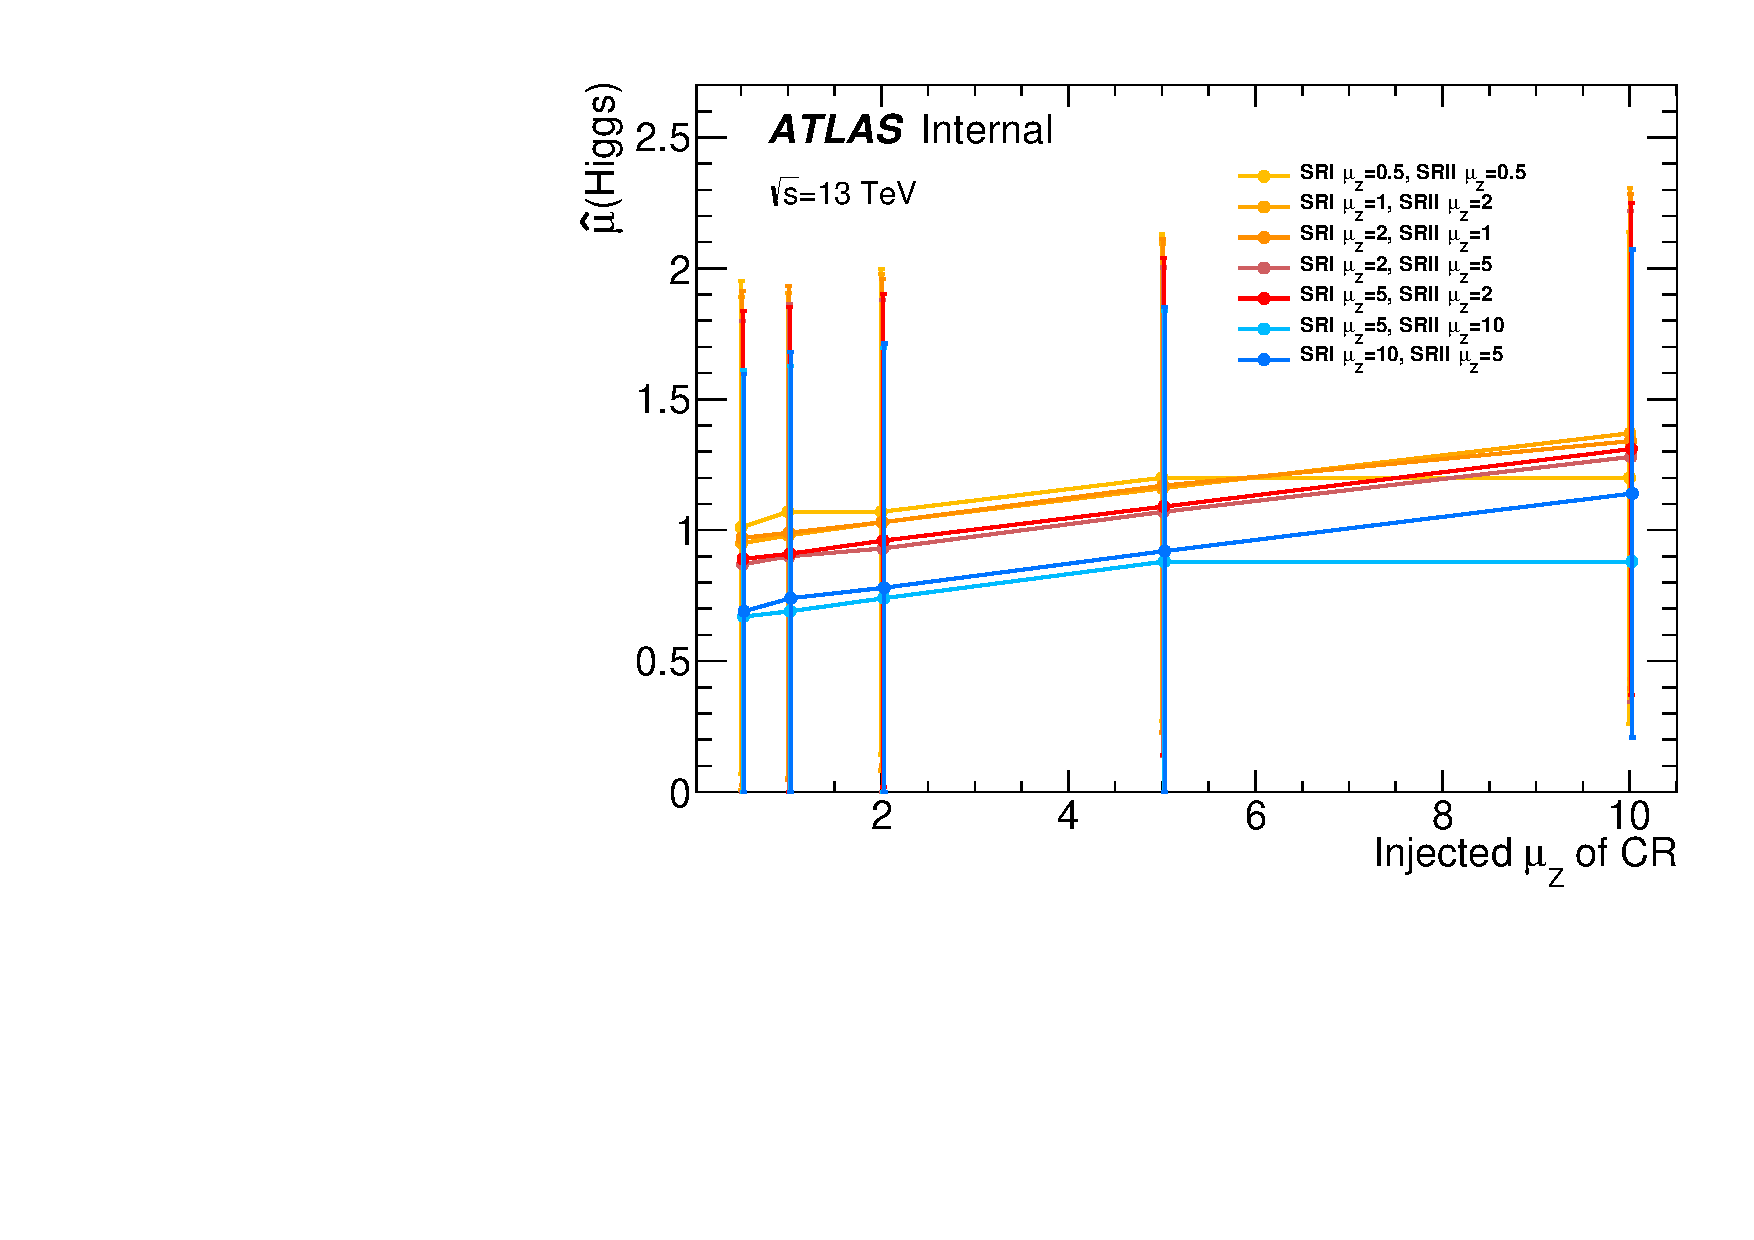
\includegraphics[width=0.48\textwidth]{figures/zstudy/zfloat_mu_CR.pdf}\\

\caption{Asimov data fit of Z-injection test applying floating the overall $Z$ normalization in \twocentral channel.}
  \label{fig:zinjection_Float}
\end{figure}


\begin{figure}[htbp]
  \centering
 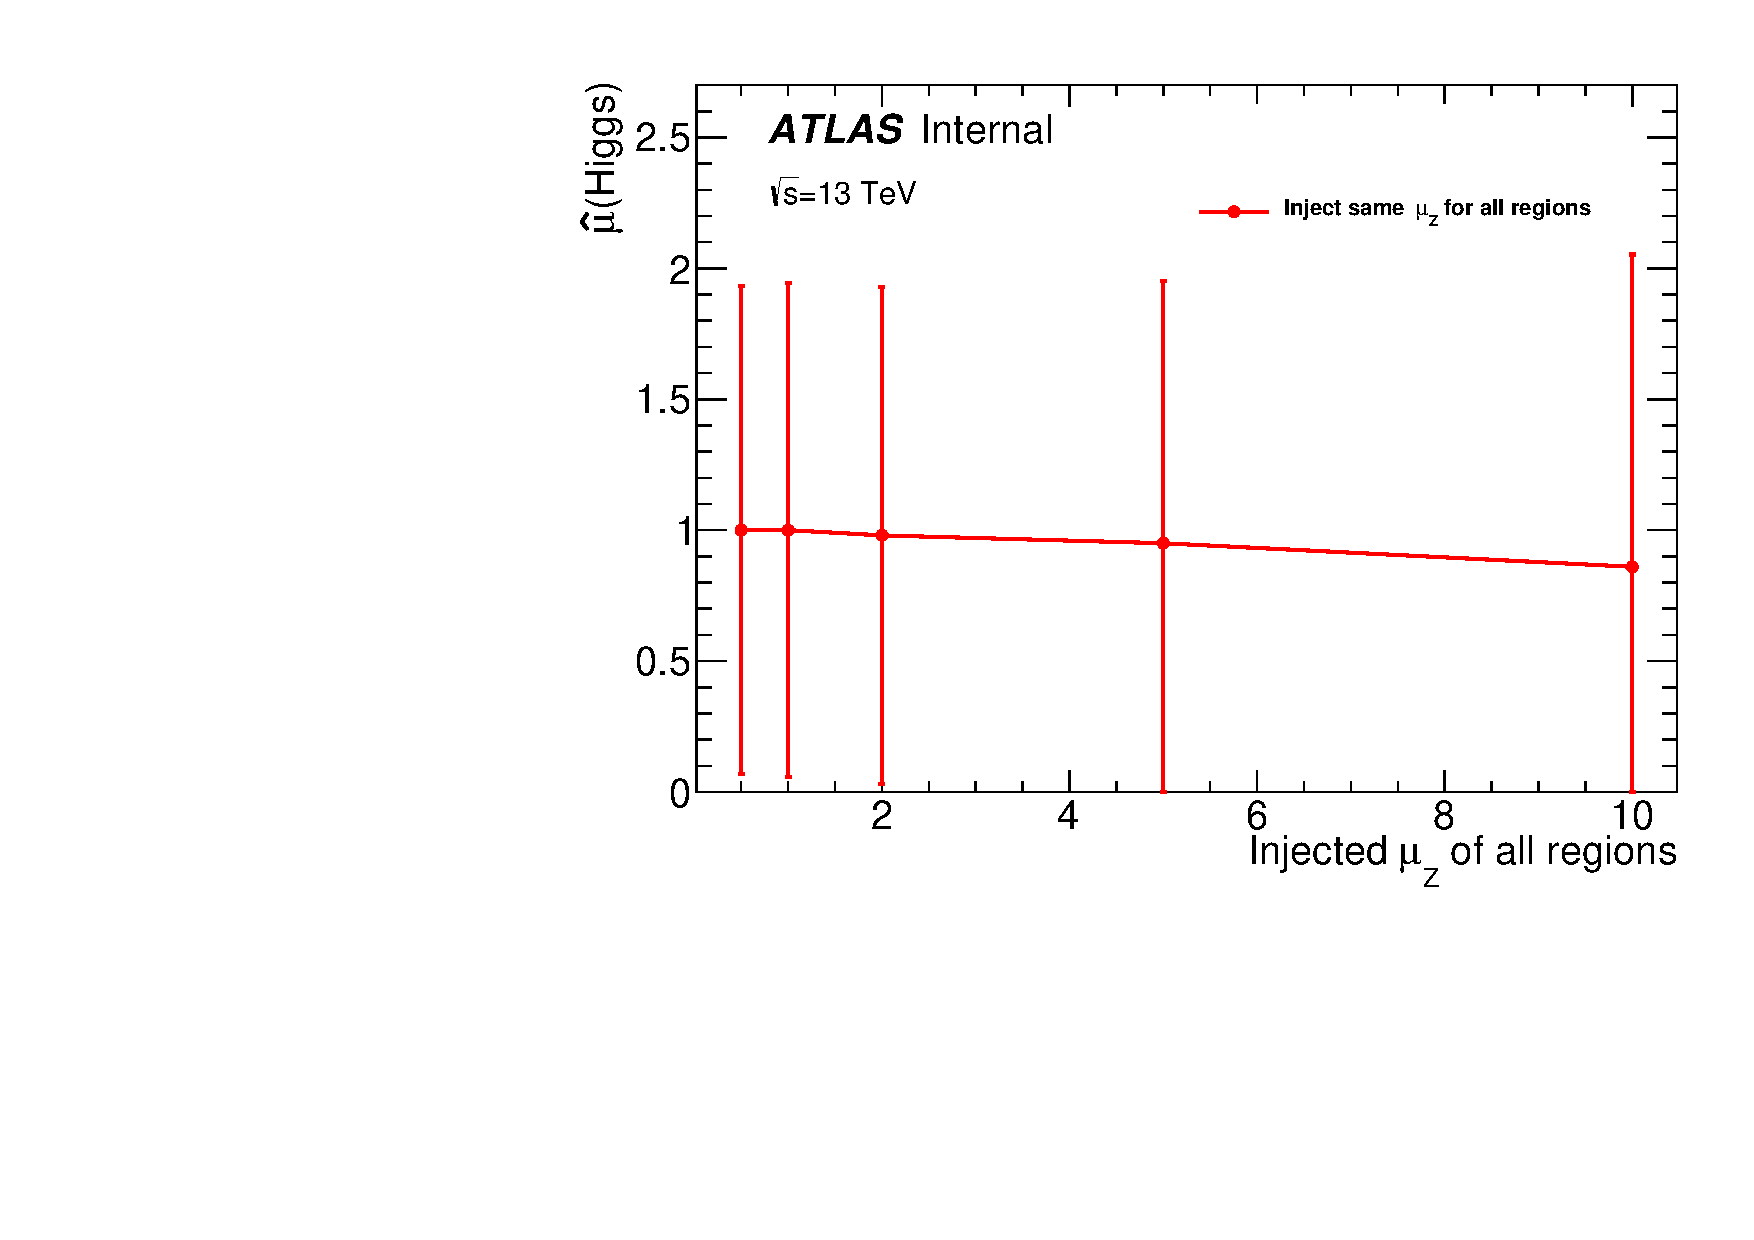
\includegraphics[width=0.48\textwidth]{figures/zstudy/zconall_mu_uniform.pdf}
 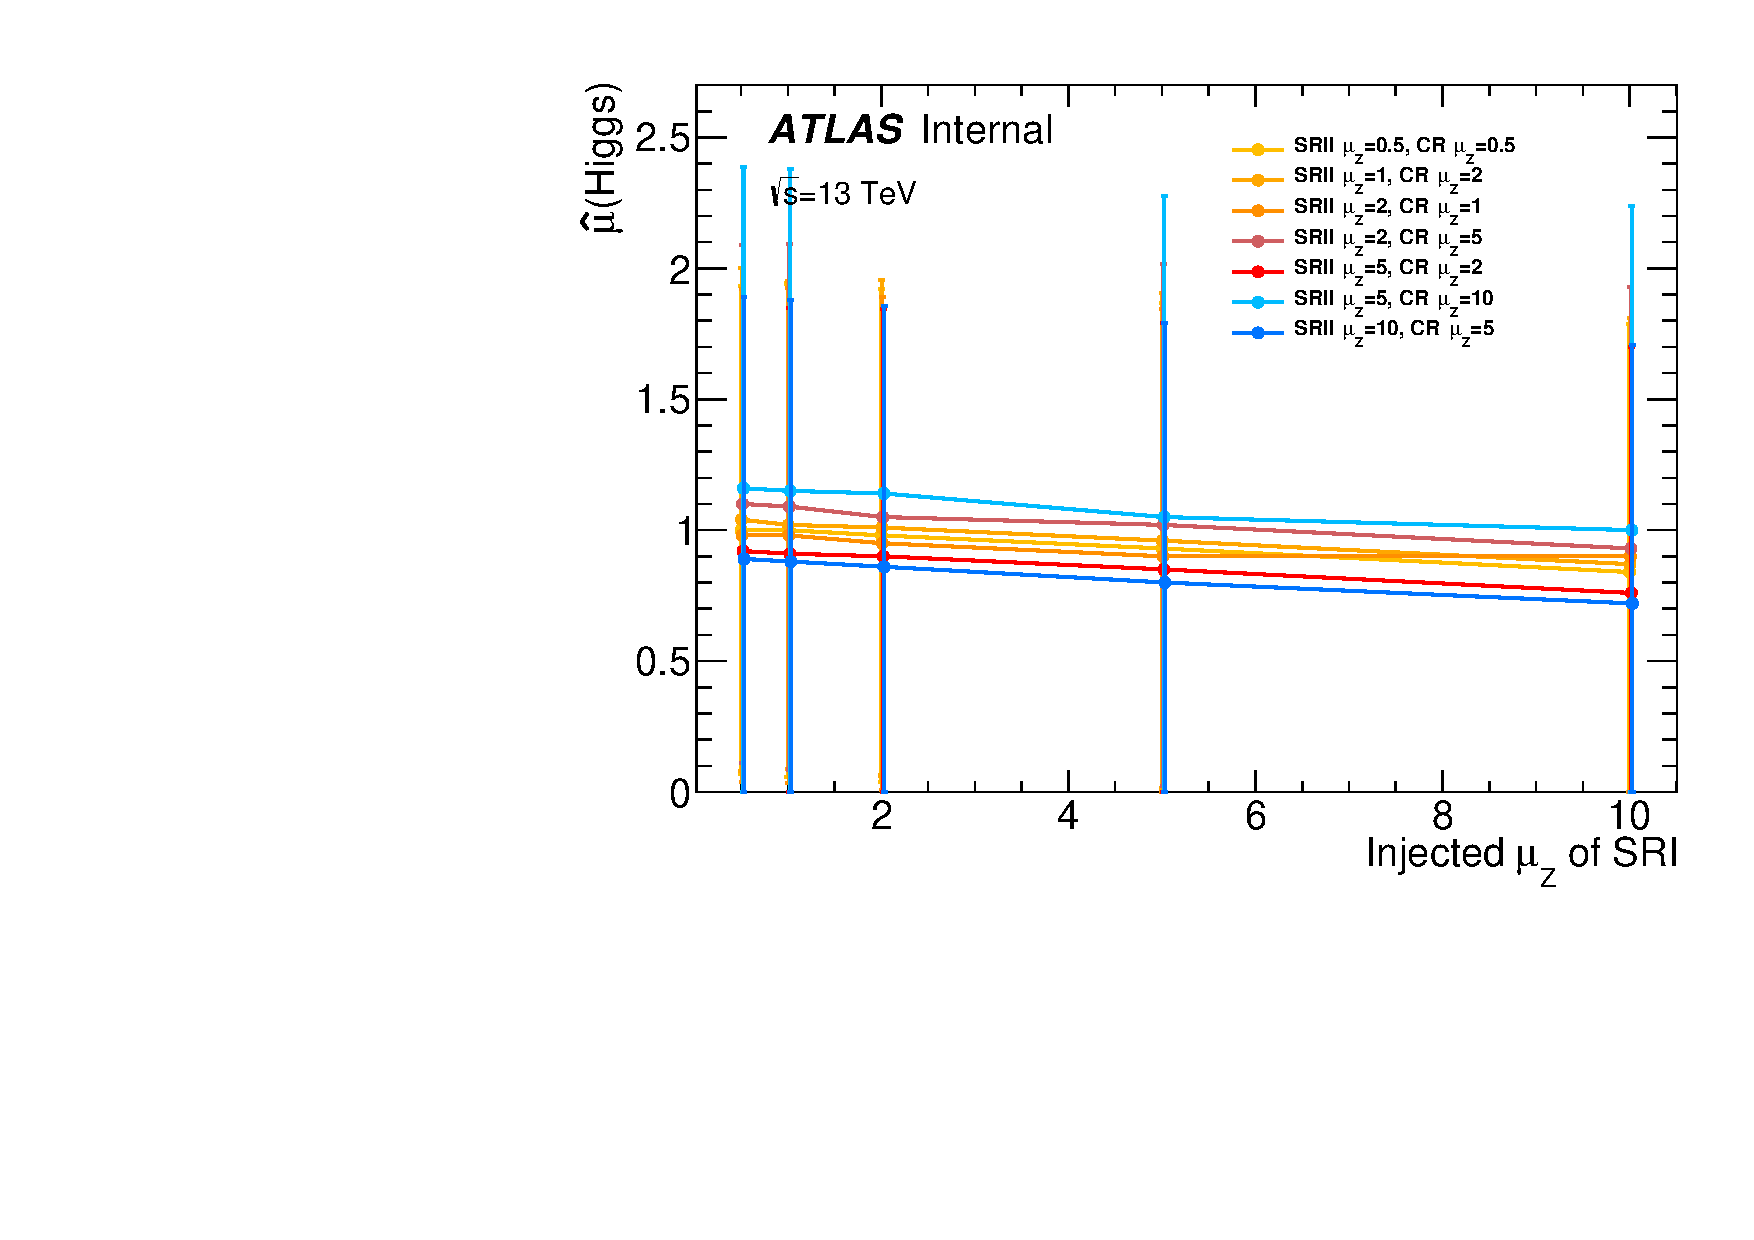
\includegraphics[width=0.48\textwidth]{figures/zstudy/zconall_mu_SRI.pdf}\\
 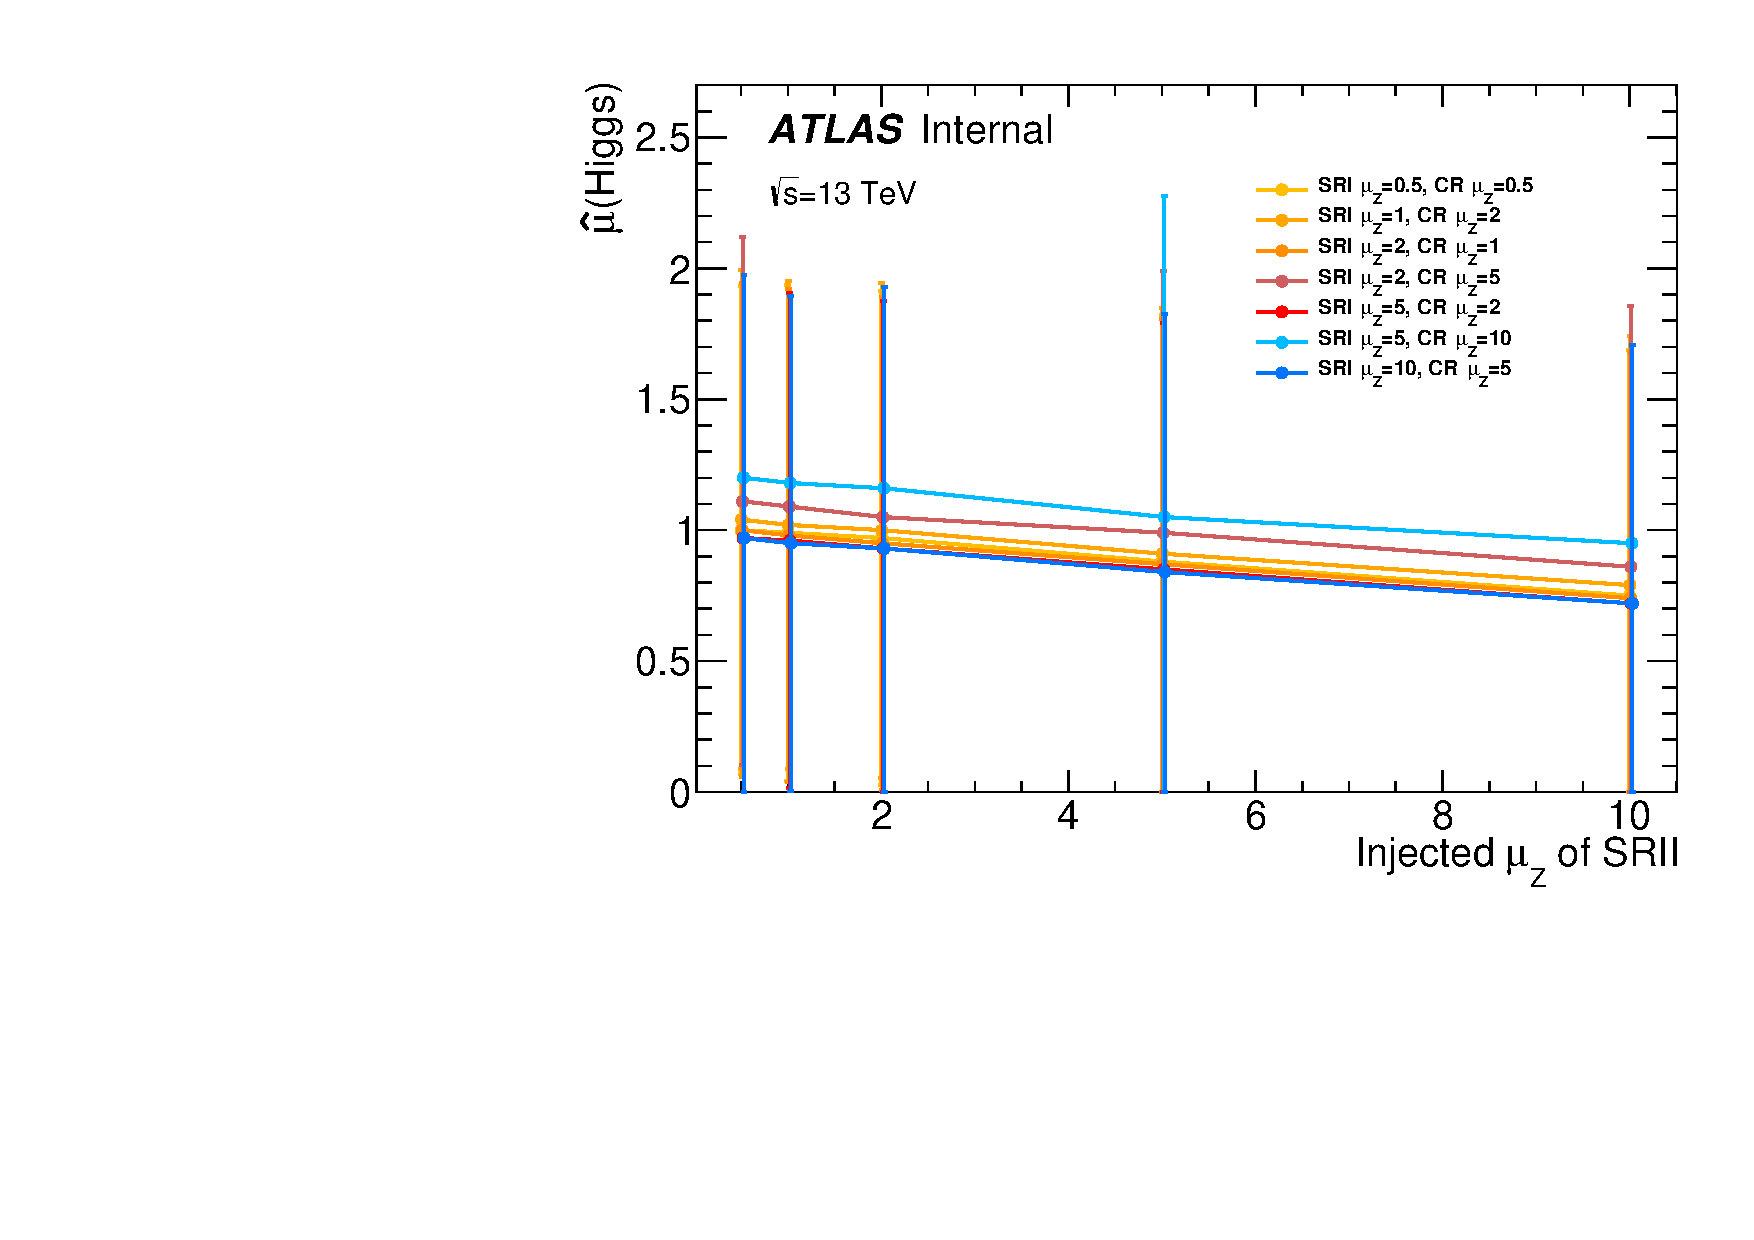
\includegraphics[width=0.48\textwidth]{figures/zstudy/zconall_mu_SRII.pdf}
 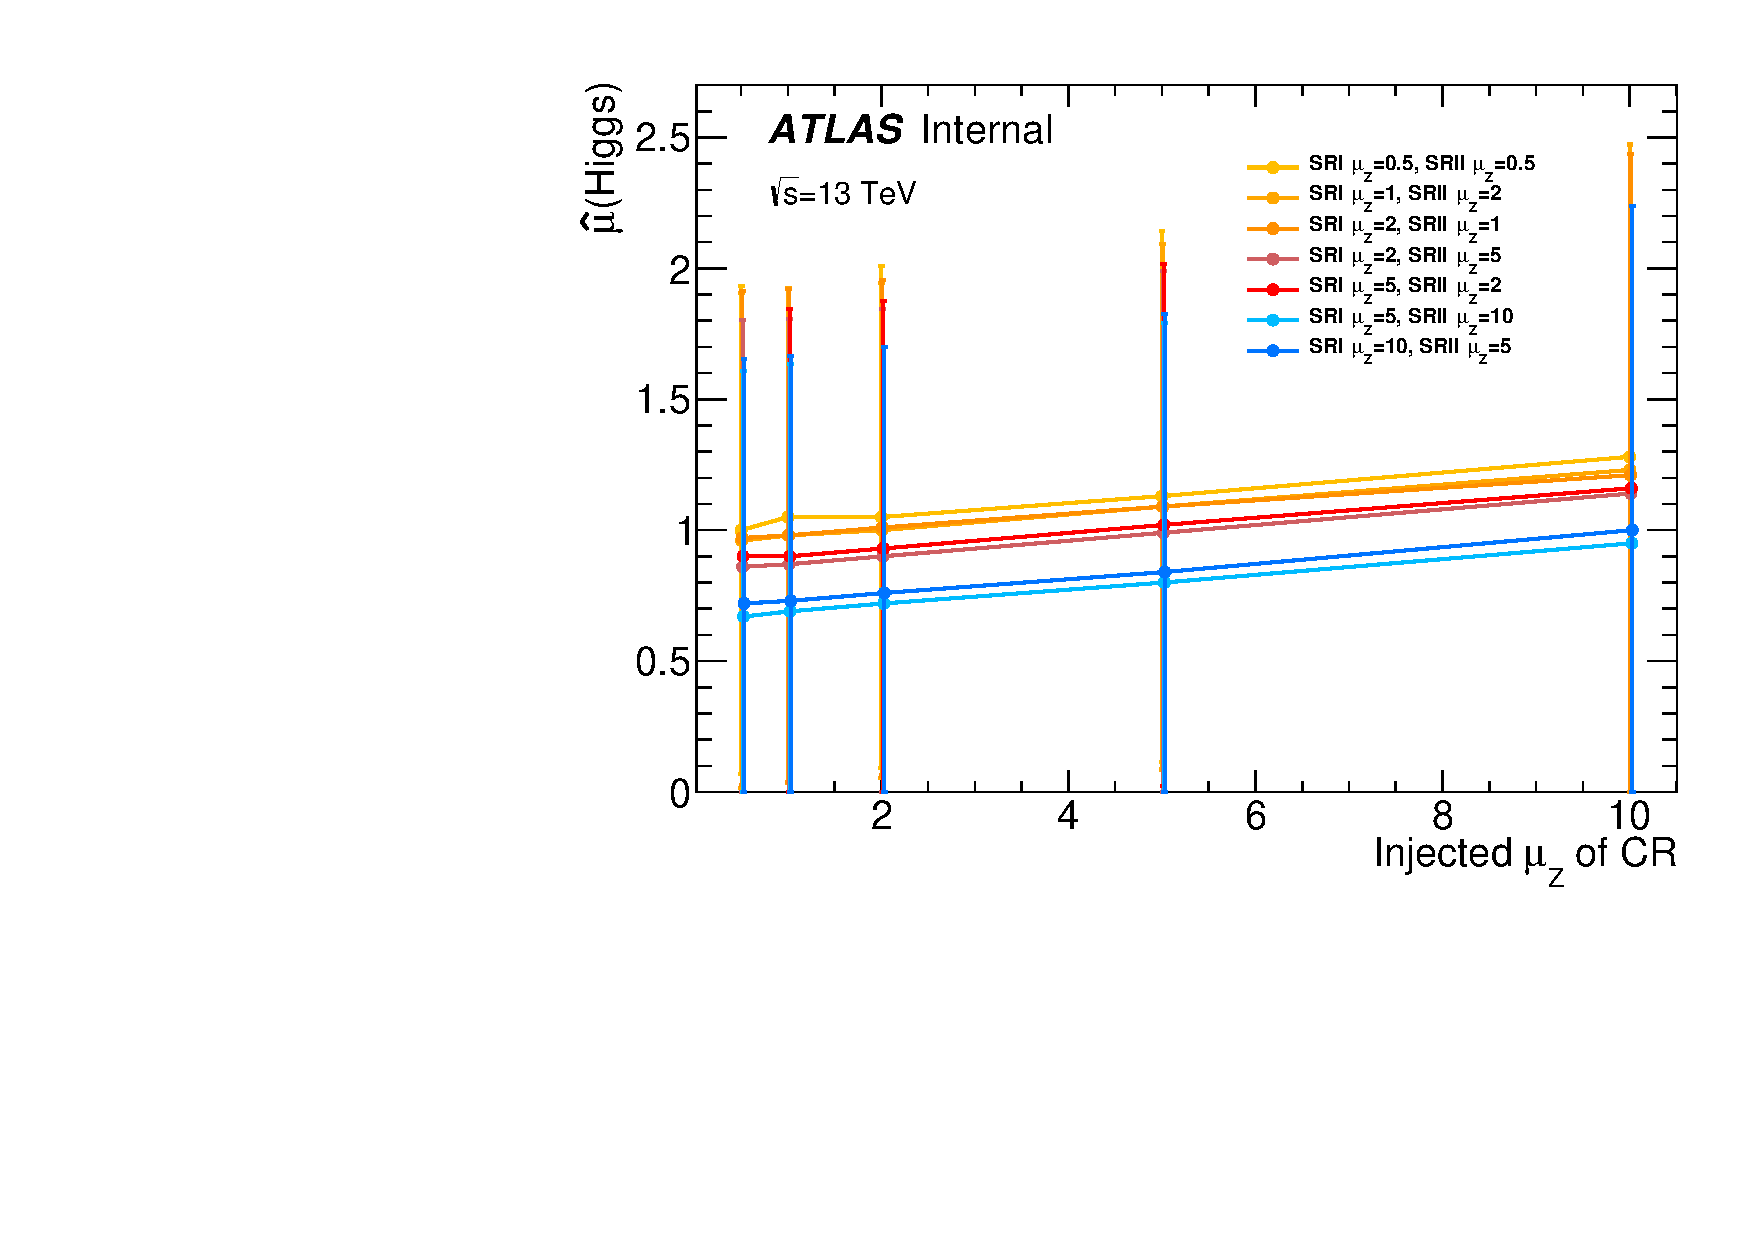
\includegraphics[width=0.48\textwidth]{figures/zstudy/zconall_mu_CR.pdf}\\

\caption{Asimov data fit of Z-injection test applying separate NPs with Gaussian prior to $Z$ normalization in each BDT regions in \twocentral channel.}
  \label{fig:zinjection_ConAll}
\end{figure}


\begin{figure}[htbp]
  \centering
 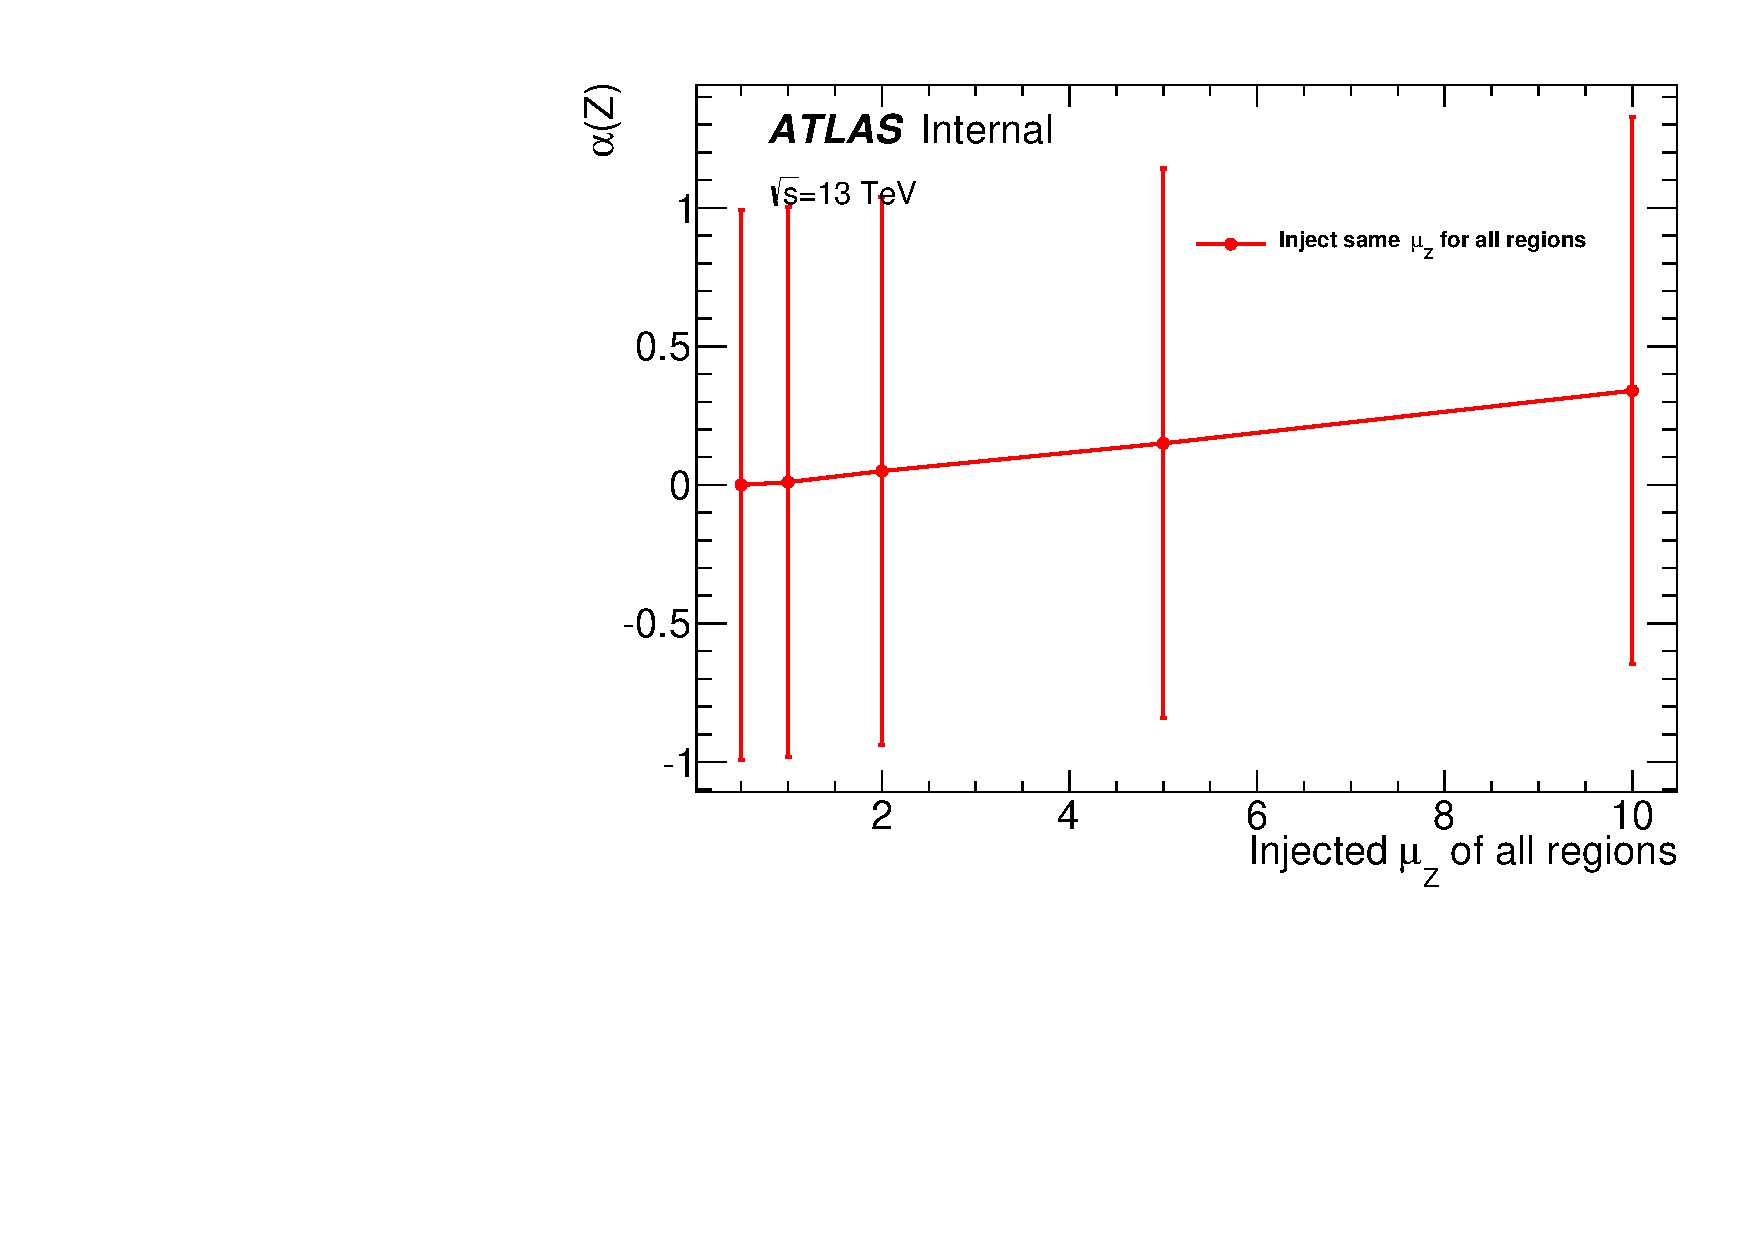
\includegraphics[width=0.48\textwidth]{figures/zstudy/zcon_alphaZ.pdf}
 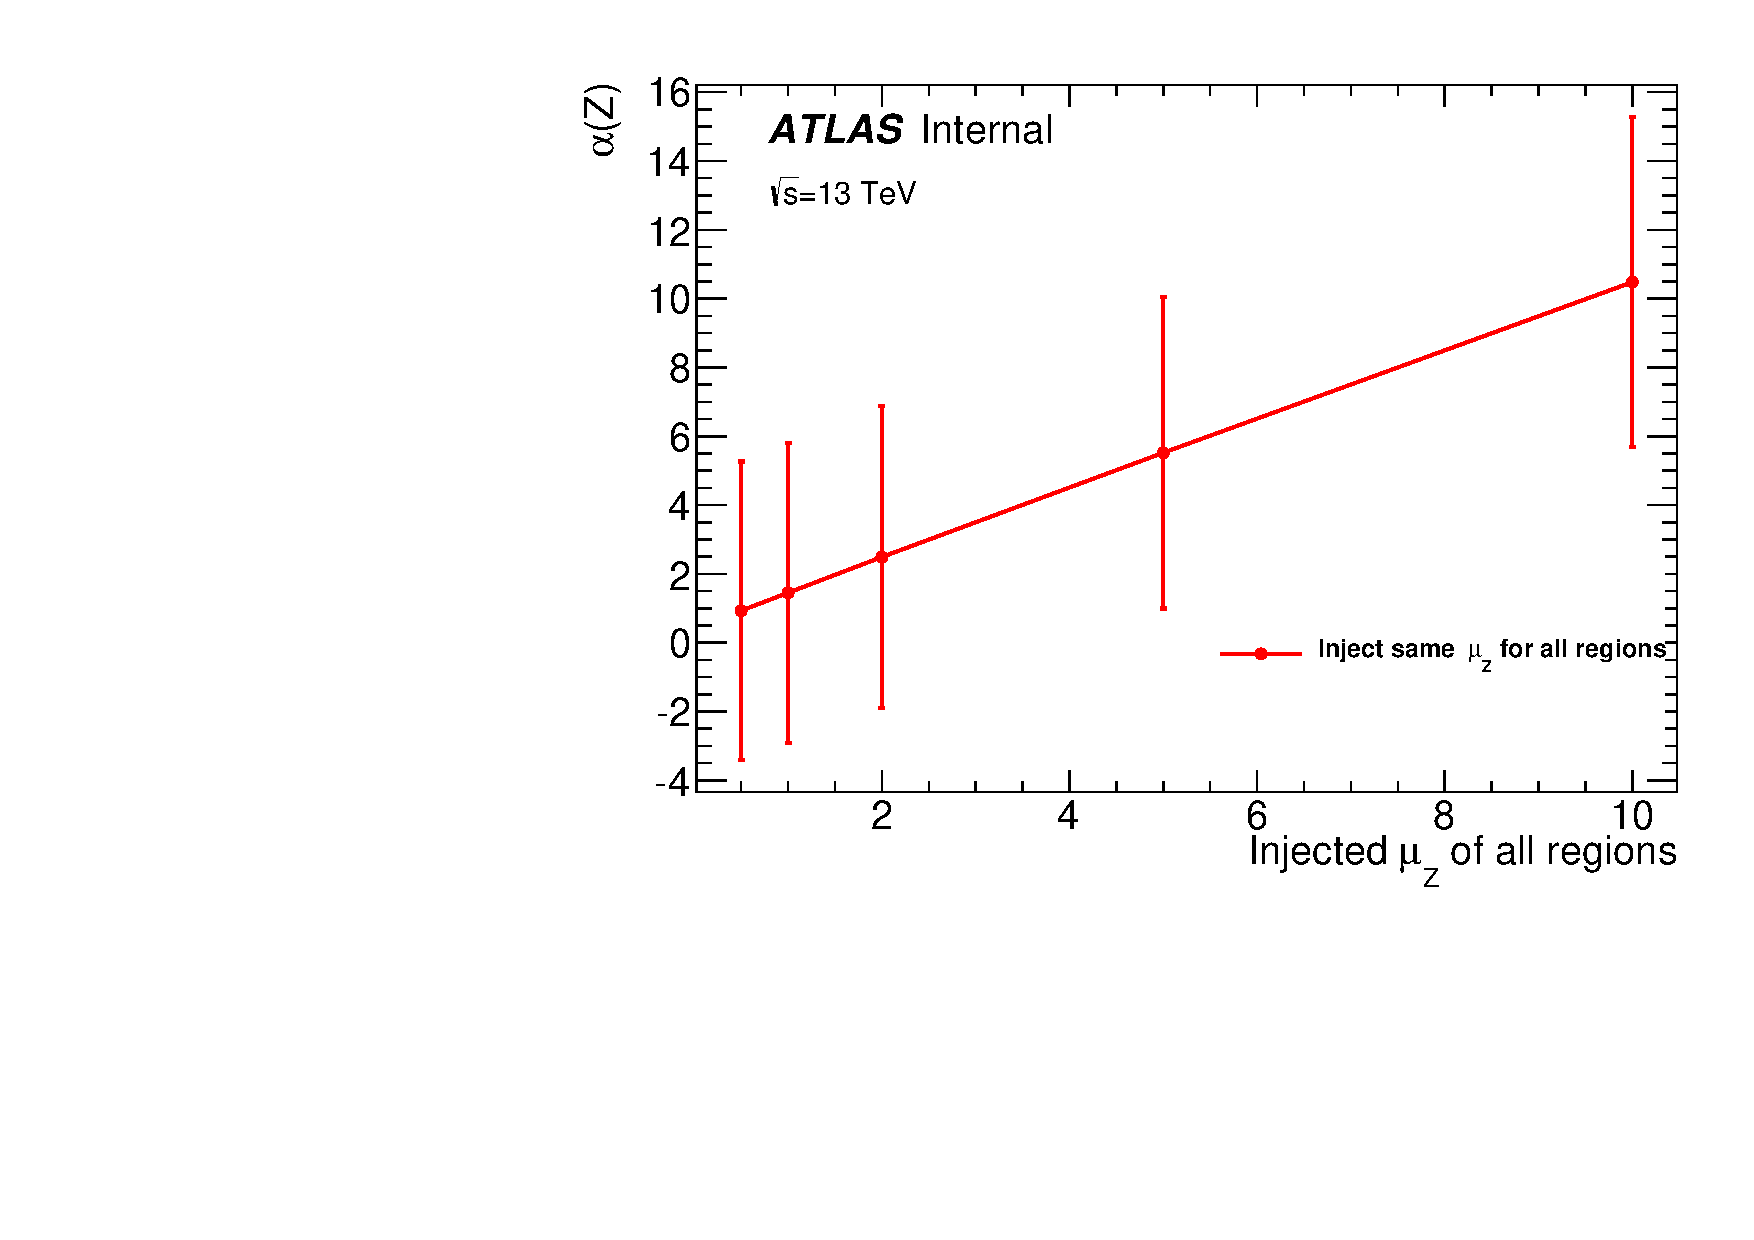
\includegraphics[width=0.48\textwidth]{figures/zstudy/zfloat_alphaZ.pdf}\\

\caption{Nuisance parameter value of $Z$ normalization of Asimov Z-injection fit in \twocentral channel. The $\alpha_{Z}$ value is constrained with a Gaussian prior (left) and left to float (right) in the fit.}
  \label{fig:zmu}
\end{figure}
